\documentclass[12pt,a4paper]{report}
\usepackage[margin=2.5cm]{geometry}
\usepackage{graphicx}
\usepackage{float}
\usepackage{subcaption}
\usepackage{booktabs}
\usepackage{parskip}
\usepackage{amsmath}
\usepackage{amssymb}
\usepackage{cleveref}
\usepackage{gensymb}
\usepackage{biblatex}
\usepackage{multirow}
\usepackage{tikz}
\usepackage{bm}
\usetikzlibrary{shapes.geometric, arrows.meta, positioning}

% Place chapter titles at the very top of the page (remove default top gap).
\usepackage{titlesec}
\titleformat{\chapter}[hang]
  {\normalfont\Large\bfseries}{\thechapter}{1em}{}
\titlespacing*{\chapter}{0pt}{0pt}{20pt}

% Look for figures in each chapter's source directory.
\graphicspath{{../energy/}{../frequency_recovery/}{../equalisation}}

% Both chapters carry their own bibliography file.  biblatex merges them;
% duplicate keys (if any) are resolved by biber to the first definition.
\addbibresource{../energy/ref.bib}
\addbibresource{../frequency_recovery/ref.bib}
\addbibresource{../equalisation/ref.bib}
\addbibresource{../clk_recovery/ref.bib}
\addbibresource{ref.bib}

\title{Energy-Efficient 200 Gbit/s Transceivers for Optical Access Networks}
\author{Joe Leacy}

\begin{document}

% =====================================================================
% Department of Engineering cover sheet (converted from coversheet.docx)
% Requires: graphicx, xcolor (provided by the tikz package in full.tex)
% =====================================================================
\begin{titlepage}
\thispagestyle{empty}
\definecolor{deptblue}{HTML}{17365D}

% --- University of Cambridge crest ---------------------------------
\noindent
\includegraphics[width=6cm]{cambridge_logo.png}

\vspace{0.4cm}
\noindent{\sffamily\Large\bfseries\color{deptblue}Department of Engineering}

% --- Title box (against right margin) ------------------------------
\vspace{3.5cm}
\begin{flushright}
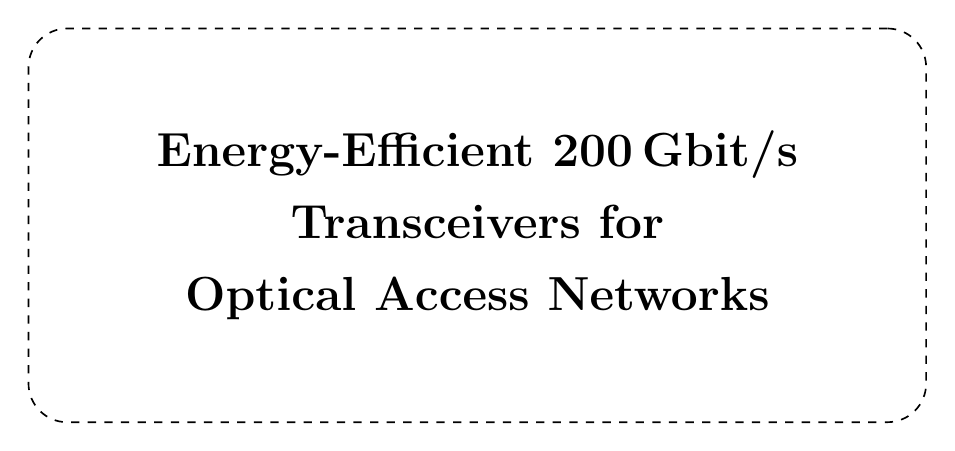
\begin{tikzpicture}
  \node[draw, dashed, rounded corners=14pt, line width=0.6pt,
        minimum width=11.4cm, minimum height=5cm,
        text width=10.5cm, align=center,
        font=\fontsize{19}{26}\selectfont\bfseries]
       {Energy-Efficient 200\,Gbit/s\\ Transceivers for\\ Optical Access Networks};
\end{tikzpicture}
\end{flushright}

% --- Author / supervisor / date (against right margin) -------------
\vspace{1.5cm}
\begin{flushright}
\begin{tabular}{rl}
  \large Author Name: & \large Joe Leacy \\[0.8em]
  \large Supervisor:  & \large Seb Savory \\[0.8em]
  \large Date:        & \large 01/06/2026 \\
\end{tabular}
\end{flushright}

% --- Declaration (at the very bottom of the page) ------------------
\vfill
\noindent I hereby declare that, except where specifically indicated, the work
submitted herein is my own original work.

\vspace{1.5cm}
\noindent Signed \underline{\makebox[6cm][l]{\,Joe Leacy}}\hfill
date \underline{\makebox[6cm][l]{\,01/06/2026}}
\end{titlepage}


\begin{abstract}
Optical access networks form the final link between an operator's exchange and the end user, and the bandwidth they must carry is growing rapidly with video, cloud, and mobile traffic. Passive optical networks (PONs), in which a single line terminal serves many subscribers through passive splitters, keep this last mile inexpensive, and coherent detection is a promising way to push them to higher data rates by recovering both the amplitude and phase of the optical field. Coherent reception, however, depends on energy-intensive digital signal processing (DSP), and because a receiver is deployed at every subscriber its energy efficiency is a primary design constraint. This project investigates the algorithm and arithmetic-precision choices that reduce the energy of a coherent passive optical network (CPON) receiver while still meeting its performance requirements.

A complete DP-QPSK receiver pipeline (chromatic-dispersion equalisation, timing recovery, adaptive equalisation, and carrier recovery) was implemented in both floating and fixed point, with each stage compiled to a bit-accurate executable model. The model estimates energy from the real operation counts and word lengths of each block and, by measuring the bit-error rate directly, captures the effect of quantisation rather than assuming it; the required SNR (RSNR) to reach the forward-error-correction threshold is used as a common figure of merit, so that the cost of a lower-energy implementation can be expressed as an SNR penalty and weighed against its energy saving. At each stage the algorithms common in long-haul systems were compared against simpler alternatives suited to a short-reach, energy-constrained link. For timing recovery, a Modified Godard detector that reuses the equaliser's FFT was shown to perform as well as a Gardner loop while avoiding the cost of a separate interpolator. For frequency recovery, a data-aided differential-phase-and-Kay estimator reached an acceptable residual offset with far fewer operations than a Rife \& Boorstyn FFT search, and for phase recovery a pilots-only correction matched the performance of the Viterbi \& Viterbi algorithm at a fraction of the cost. The minimum viable fixed-point precision of each stage was found and the combined operating points evaluated end to end. The static equaliser was found to dominate the receiver energy, making equaliser precision and power-of-two twiddle-factor rounding the most effective means of reducing it, and converting each implementation's RSNR into a transmitter energy through a shot-noise network model indicated that the receiver dominates the combined system energy at the operating points considered. These results are presented as a comparison between implementations rather than as absolute figures, given the simplifications in the energy and network models.
\end{abstract}

\tableofcontents

% =====================================================================
\chapter{Access Networks and Coherent PON}\label{chapter:cpon}
% =====================================================================

\section{Optical Access Networks}
The access network is the final link between an operator's central exchange and the end user, often called the \emph{last mile}. Exponentially growing bandwidth demands from streaming, cloud services, and 5G backhaul are placing severe pressure on this segment. 

A passive optical network (PON) uses a point-to-multipoint (P2MP) topology in which a single optical line terminal (OLT) at the exchange serves multiple optical network units (ONUs) at the customer premises through a tree of passive optical splitters, as illustrated in \cref{fig:pon_intro}. No active components are required in the distribution plant, keeping operational costs low.

\begin{figure}[H]
    \centering
    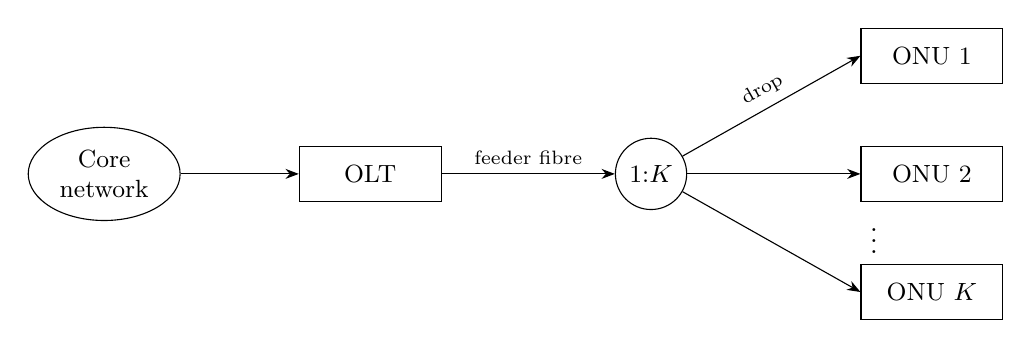
\begin{tikzpicture}[
        box/.style={draw, rectangle, minimum width=1.8cm, minimum height=0.7cm, align=center, font=\small},
        cloud/.style={draw, ellipse, minimum width=1.6cm, minimum height=0.9cm, align=center, font=\small},
        spl/.style={draw, circle, minimum size=0.9cm, align=center, font=\small},
        node distance=0pt
    ]
        \node[cloud] (net) {Core\\network};
        \node[box, right=1.5cm of net] (olt) {OLT};
        \node[spl, right=2.2cm of olt] (s1) {\small 1:$K$};
        \draw[-{Stealth}] (net) -- (olt);
        \draw[-{Stealth}] (olt) -- node[above]{\scriptsize feeder fibre} (s1);

        \node[box, right=2.2cm of s1, yshift= 1.5cm] (onu1) {ONU 1};
        \node[box, right=2.2cm of s1, yshift= 0.0cm] (onu2) {ONU 2};
        \node[right=2.2cm of s1, yshift=-0.75cm] (dots) {$\vdots$};
        \node[box, right=2.2cm of s1, yshift=-1.5cm] (onuk) {ONU $K$};

        \draw[-{Stealth}] (s1) -- node[above, sloped]{\scriptsize drop} (onu1.west);
        \draw[-{Stealth}] (s1) -- (onu2.west);
        \draw[-{Stealth}] (s1) -- (onuk.west);
    \end{tikzpicture}
    \caption{Passive optical network: one OLT serves $K$ ONUs via a passive 1:$K$ splitter.}
    \label{fig:pon_intro}
\end{figure}

\section{Coherent PON}
Traditional intensity-modulation direct-detection (IM-DD) passive optical networks are reaching their practical limits at data rates around 50 Gbit/s per wavelength. Coherent technology encodes information in the amplitude and phase of the optical signal, allowing modulation formats such as QPSK that can carry more bits per symbol. Coherent receivers are also more sensitive, allowing for lower transmit powers. These factors make them a promising alternative to achieve rates of 200 Gbit/s on an acceptable power budget \cite{Faruk;21}.


\section{Specification}
The Coherent Passive Optical Network (CPON) specification \cite{CPON_PMD_2025} defines a single-wavelength P2MP system and serves as the reference specification for the receiver implementations evaluated in this report. This report focuses on the \emph{downstream} direction (OLT to ONU) where receiver optimisations can be shared by all ONUs; the key physical-layer parameters are described in the following sections.

\subsection{Modulation and Symbol Rate}
The downstream signal uses non-differential dual-polarisation QPSK (DP-QPSK) at a symbol rate of $R_s = 30.5$\,GBd. Each polarisation carries 2\,bits per symbol by mapping consecutive bit pairs to in-phase and quadrature amplitudes $I,Q\in\{-1,+1\}$, giving QPSK constellation points at $\pm1\pm j$. Training and pilot symbols use the same QPSK constellation as the data symbols. Soft-decision forward error correction (FEC) is used with a 22\% coding overhead.

\subsection{Downstream Frame Structure}
\label{sec:cpon_frame}

The fundamental framing unit is the \emph{DSP subframe} of 3\,712 symbols, organised as $116\times32$-symbol blocks. Every block begins with a pilot symbol; the first block also carries an 11-symbol training sequence, whose first symbol doubles as pilot index~1.

\subsection{Key System Tolerances}
\label{sec:cpon_tolerances}

The key physical-layer tolerances that the receiver DSP must accommodate are summarised in \cref{tab:cpon_tolerances}. The transmitter SNR of 35\,dB is the back-to-back signal quality at the OLT, accounting for impairments in the core network before the access link, and sets the noise floor $\mathrm{NSR}_0$ used in the transmitter-energy model of \cref{chapter:energy}. The worst-case values of \cref{tab:cpon_tolerances} are used in each experiment.

\begin{table}[H]
    \centering
    \small
    \caption{Key downstream tolerances from the CPON specification \cite{CPON_PMD_2025}.}
    \label{tab:cpon_tolerances}
    \begin{tabular}{lc}
        \toprule
        Parameter & Value \\
        \midrule
        Loss budget (OLT to ONU)        & $35$\,dB \\
        Transmitter SNR                 & $35$\,dB \\
        Worst-case CFO                  & $\approx 3$\,GHz \\
        Laser linewidth (OLT and ONU)   & $\leq 1$\,MHz \\
        Sampling frequency offset (SFO) & $\leq 40$\,ppm \\
        Chromatic dispersion            & $\leq 1600$\,ps/nm \\
        Polarisation-mode dispersion    & $\leq 8$\,ps \\
        Reach                           & $\leq 80$\,km \\
        \bottomrule
    \end{tabular}
\end{table}

The specification requires a pre-FEC bit error ratio of $\leq 2\times10^{-2}$, which the soft-decision LDPC FEC reduces to a post-FEC BER of $\leq10^{-12}$.

% =====================================================================
\chapter{Network and Receiver Models}\label{chapter:energy}
% =====================================================================

\section{Simulation Framework}
All DSP algorithms in this report are designed, characterised, and compared through software simulation in MATLAB. The simulated receiver processes DP-QPSK symbols generated at the CPON downstream parameters described in \cref{chapter:cpon}. The receiver follows the standard coherent-DSP pipeline shown in \cref{fig:receiver_pipeline}.

\begin{figure}[H]
    \centering
    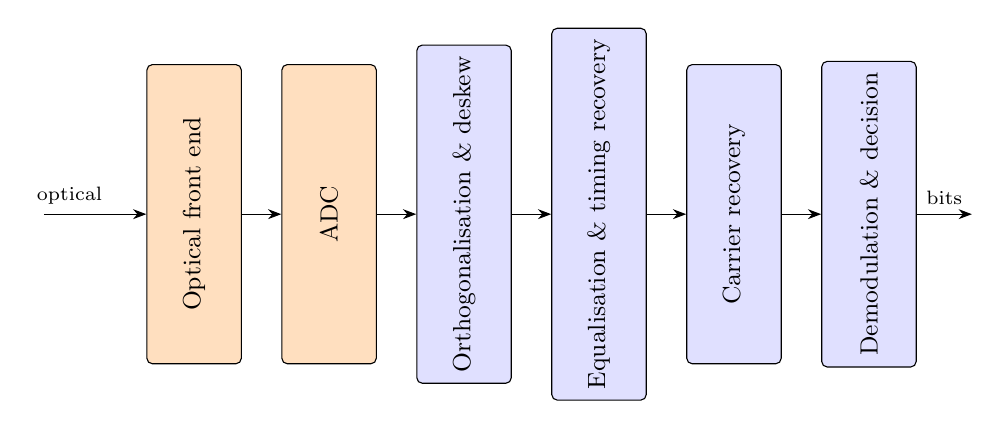
\begin{tikzpicture}[
        stage/.style={draw, rectangle, rounded corners=2pt, fill=blue!12, minimum width=1.2cm, minimum height=3.8cm, align=center, font=\small, inner sep=4pt},
        analog/.style={stage, fill=orange!25},
        node distance=0.4cm and 0.5cm
    ]
        \node[analog] (fe)   {\rotatebox{90}{Optical front end}};
        \node[analog, right=of fe]   (adc)  {\rotatebox{90}{ADC}};
        \node[stage, right=of adc]  (orth) {\rotatebox{90}{Orthogonalisation \& deskew}};
        \node[stage, right=of orth] (eq)   {\rotatebox{90}{Equalisation \& timing recovery}};
        \node[stage, right=of eq]   (cr)   {\rotatebox{90}{Carrier recovery}};
        \node[stage, right=of cr]   (dec)  {\rotatebox{90}{Demodulation \& decision}};

        \draw[-{Stealth}] ([xshift=-1.3cm]fe.west) -- node[above, font=\scriptsize, pos=0.25]{optical} (fe.west);
        \draw[-{Stealth}] (fe)   -- (adc);
        \draw[-{Stealth}] (adc)  -- (orth);
        \draw[-{Stealth}] (orth) -- (eq);
        \draw[-{Stealth}] (eq)   -- (cr);
        \draw[-{Stealth}] (cr)   -- (dec);
        \draw[-{Stealth}] (dec.east) -- node[above, font=\scriptsize]{bits} ++(0.7cm,0);
    \end{tikzpicture}
    \caption{DSP pipeline of the simulated coherent receiver. The analogue stages (orange) and the digital stages (blue) are distinguished by colour. The optical front end mixes the received signal with a local-oscillator laser to produce four baseband photocurrents, which the ADCs digitise; orthogonalisation and deskew correct front-end imbalances; equalisation and timing recovery compensate the linear channel and recover the symbol-rate sampling phase; carrier recovery removes the residual CFO and laser phase noise; the final stage maps each symbol to bits.}
    \label{fig:receiver_pipeline}
\end{figure}

\subsection{Fixed-Point Arithmetic}
The receiver is evaluated with fixed-point arithmetic, as used in ASIC designs. This captures the effect of quantisation error on each implementation's performance, and underpins a bit-accurate energy model that goes beyond algorithmic complexity. All fixed-point modelling uses the MATLAB Fixed-Point Designer toolkit.

Fixed-point values require a well-defined range that they represent. The range of the input signal can vary due to additive noise and dispersive effects so normalisation to the range [-1,1] on the real and imaginary axes is first performed before further processing. The normalisation must balance some points exceeding the range and saturating with points being compressed to the centre. A suitable approach found by trial-and-error is the linear rescaling by the signal magnitude at the 99th percentile with larger amplitudes saturating.

\section{Energy Estimation}
The energy-efficiency of a receiver implementation cannot be determined from the receiver energy alone. A simpler architecture may reduce receiver energy but, through a drop in accuracy, incur an SNR penalty that raises the transmit power needed for acceptable operation. This calls for a system-level model of the energy consumption where an SNR penalty can be converted to an equivalent increase in transmitter energy, allowing receiver implementations to be compared by their combined energy.
\subsection{Receiver Energy}\label{sec:rx_energy}
The energy consumption of the receiver can be estimated from the number of real multiplications \(N_M\) and real additions \(N_A\) it performs to process each symbol. The true cost of these operations depends on the hardware implementation. The reference values shown in \cref{tab:energy} provide a useful estimate to compare DSP algorithms but a more accurate estimate would require power simulations for an ASIC implementation.

\begin{table}[H]
    \centering
    \caption{Energy cost of arithmetic operations for different bit widths in 45\,nm CMOS \cite{horowitz2014computing}.}
    \label{tab:energy}
    \begin{tabular}{ccc}
        \toprule
        \(n\) (bits) & Add (pJ) & Multiply (pJ) \\
        \midrule
        8  & 0.03 & 0.2 \\
        32 & 0.1  & 3.1 \\
        \bottomrule
    \end{tabular}
\end{table}

\paragraph{Dependence on Word Length}
A ripple-carry adder performs \(n\) bit-wise additions on words of length \(n\), so its energy scales linearly with \(n\). A shift-and-add multiplier accumulates \(n\) partial products of length \(n\) and so scales as \(n^2\). Modern adders and multipliers (e.g.\ carry-lookahead, Booth/Wallace) reduce these costs by a constant factor or to $n\log n$, so the scalings used here are upper bounds; comparisons between algorithms remain valid because all are penalised equally. The proportionality constants are calibrated by a least-squares fit through the origin to the two data points of \cref{tab:energy}, giving
\begin{equation}
    E_A(n) = 3.16\,n \mathrm{\ fJ}, \qquad E_M(n) = 3.03\,n^2 \mathrm{\ fJ}.
    \label{eq:arithmetic_45}
\end{equation}
Energy consumption for arithmetic operations in modern process nodes is not widely reported, and Dennard scaling (the rule that transistor power density remained constant as they were scaled down) \cite{Esmaeilzadeh;11} can no longer be applied to extrapolate from the values in \cref{tab:energy}. As an approximation, the $\approx 75\%$ reduction in total power dissipation at constant frequency reported for an Intel core moving from 45\,nm to 14\,nm CMOS \cite{Shahidi;19} is taken as a proxy for the per-operation energy scaling. This conflates contributions from leakage, clocks, caches and I/O with the arithmetic energy of interest, so the resulting numbers should be read as an estimate rather than a calibrated figure. Applying this reduction to the 45\,nm fit gives
\begin{equation}
    E_A(n) = 0.79\,n \mathrm{\ fJ}, \qquad E_M(n) = 0.76\,n^2 \mathrm{\ fJ}.
    \label{eq:arithmetic_14}
\end{equation}
\paragraph{Amortisation}
Some DSP algorithms perform computations that are reused over multiple symbols. For example, carrier frequency offset (CFO) varies much slower than the symbol rate so can be estimated less frequently. For a computation that requires \(N_M\) multiplications and \(N_A\) additions and is used by \(S\) symbols, the operations per symbol would be \(N_M / S\) and \(N_A / S\).

\paragraph{CORDIC}
Coherent receivers perform phase estimates and rotations on complex-valued data in several DSP blocks. This is done efficiently in fixed-point hardware with the CORDIC algorithm, which evaluates these operations using only shifts and additions. CORDIC iteratively rotates a vector by the fixed angles \(\arctan(2^{-i})\), each implemented as a bit-shift and an add/subtract. Each iteration adds roughly one bit of angular resolution, so $n$ bits of precision require $n$ CORDIC iterations and the cost is taken to be equivalent to an $n$-bit real multiplication.

\paragraph{Total Energy and Power}
Many DSP blocks operate on complex-valued data; each complex multiplication is counted as 4 real multiplications and 2 real additions, and each complex addition as 2 real additions. The energy per symbol for the entire receiver is then
\begin{equation}
    E_{\mathrm{rx},s} = \sum_{k=1}^{L} 2 \left[ N_{A,k}E_A(n_k) + N_{M,k}E_M(n_k) \right],
\end{equation}
where the receiver is decomposed into \(L\) blocks that use different word lengths \(n_k\) according to their required precision, and \(N_{A,k}\), \(N_{M,k}\) are the addition and multiplication counts per symbol. The factor of 2 is for both polarisations. Blocks operating on the oversampled signal at rate \(f > R_s\) have their per-sample operation counts scaled by the oversampling ratio \(f/R_s\). The receiver power is then
\begin{equation}
    P_\mathrm{rx} = R_s E_{\mathrm{rx},s},
\end{equation}
and converting to energy per bit allows fair comparison across modulation schemes and symbol rates,
\begin{equation}
    E_\mathrm{rx} = \frac{E_{\mathrm{rx},s}}{\log_2(M)},
    \label{eq:rx_energy}
\end{equation}
where \(M\) is the modulation order.
\subsection{Transmitter Energy}
The downstream link considered here consists of a single OLT transmitting through a 1:\(K\) passive splitter to \(K\) ONUs, as shown in \cref{fig:pon_intro}. The OLT power is divided equally between branches, so each ONU receives a \(1/K\) share.

\paragraph{Minimum Required SNR}
The CPON standard specifies a maximum pre-FEC bit-error rate (BER) of \(2\times10^{-2}\) that must not be exceeded for the forward error-correction (FEC) scheme to function correctly. Each receiver implementation therefore has a minimum required SNR (RSNR) to meet this FEC threshold. This SNR, together with the noise characteristics of the optical network, determines the minimum transmitter power.

\paragraph{Noise}
The relationship between SNR and transmitter power \(P_\mathrm{tx}\) depends on the dominant source of noise in the network. Optical access networks typically operate over short lengths at low power, so amplifiers can be omitted and non-linear noise neglected, leaving shot noise as the dominant impairment. The shot noise power referred to the optical input of a balanced coherent receiver is \(2h\nu B_\mathrm{eff}\), where the factor of 2 captures the contributions from the signal and LO arms of the balanced detector summed in quadrature, and \(B_\mathrm{eff}\) is the receiver electrical bandwidth, set equal to the symbol rate by a matched bandpass filter after the 1:\(K\) splitter in \cref{fig:pon_intro}. The power per polarisation received by each ONU is \(P_\mathrm{tx}/2\Gamma K\), where $\Gamma$ is the loss from OLT to ONU. This gives a per-ONU NSR of
\begin{equation}
    \mathrm{NSR} = \frac{4\Gamma K h\nu B_\mathrm{eff}}{P_\mathrm{tx}} + \mathrm{NSR}_0,
    \label{eq:snr_shot}
\end{equation}
where $\mathrm{NSR} = 1/\mathrm{SNR}$ and $\mathrm{NSR}_0$ is the back-to-back NSR at the OLT. Rearranging gives the transmitted power as
\begin{equation}
    P_\mathrm{tx} = \frac{4\Gamma Kh\nu B_\mathrm{eff}}{\mathrm{NSR} - \mathrm{NSR}_0}.
\end{equation}
Assuming Nyquist pulse-shaping and matched bandpass filtering at the receiver ($B_\mathrm{eff} = R_s$), the energy per bit transmitted is
\begin{equation}
    E_\mathrm{tx} = \frac{P_\mathrm{tx}}{2KR_s \log_2(M)} = \frac{2\Gamma h\nu}{(\mathrm{NSR} - \mathrm{NSR}_0)\log_2(M)}.
    \label{eq:tx_bit_energy}
\end{equation}


\subsection{Combined Energy}
Before calculating a combined energy contribution, the transmitted optical energy in \cref{eq:tx_bit_energy} must be converted into an energy drawn from the electrical power supply by estimating the efficiencies of the transmitting laser and the modulator. The dual-polarisation modulator (\cref{fig:mzm}) consists of two nested-Mach-Zehnder IQ modulators sharing a common laser through a polarisation beam splitter, with their outputs recombined by a polarisation beam combiner. Each IQ modulator has the transfer function \cite{Mello;21}
\begin{equation}
    \frac{E_\mathrm{output}(t)}{E_\mathrm{input}(t)} = \frac{1}{2}\sin\left[\frac{v_I(t)\pi}{2V_\pi}\right] + \frac{j}{2}\sin\left[\frac{v_Q(t)\pi}{2V_\pi}\right],
\end{equation}
where each MZM is biased at its transmission null so that $v_I = v_Q = 0$ produces no output and the drive voltages swing symmetrically about $0\,$V.
\begin{figure}[H]
    \centering
    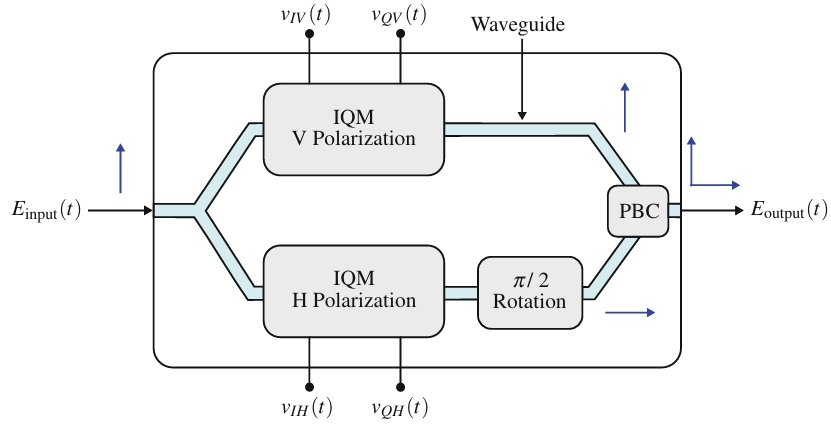
\includegraphics[width=0.65\textwidth]{MZM.jpeg}
    \caption{Dual-polarisation coherent modulator using MZMs \cite{Mello;21}.}
    \label{fig:mzm}
\end{figure}
QPSK is generated by driving each MZM between adjacent transmission peaks, $v_I(t), v_Q(t) \in \{-V_\pi, +V_\pi\}$, so
\begin{equation}
    \frac{E_\mathrm{output}(t)}{E_\mathrm{input}(t)} = \pm\frac{1}{2} \pm \frac{j}{2}
\end{equation}
and $P_\mathrm{out} = P_\mathrm{in}/2$, where the loss comes from power coupled to unused ports in the 2$\times$2 couplers. An ideal polarisation beam splitter and combiner introduce no further loss, so the \emph{marginal} efficiency of the dual-polarisation modulator is
\begin{equation}
    \eta_\mathrm{DPM} = \frac{dP_\mathrm{tx}}{dP_\mathrm{in}} = 0.5.
 \end{equation}
The overall efficiency would also include the power dissipated in the drive electronics, but this is independent of transmit power and so cancels in a comparison of receiver implementations. Combining with the wall-plug efficiency of the laser $\eta_\mathrm{WP}$ gives an overall efficiency of
\begin{equation}
    \eta_\mathrm{T} = \eta_\mathrm{WP}\eta_\mathrm{DPM} = 0.5\eta_\mathrm{WP}.
\end{equation}
Recently reported values for the wall-plug efficiency of lasers suited to coherent systems are 16-19\% \cite{Zhang;24,Vaskasi;22} which gives an overall efficiency of just under 10\%. A measure of combined energy is then
\begin{equation}
    E_\mathrm{sys} = \frac{1}{\eta_\mathrm{T}}E_\mathrm{tx} + E_\mathrm{rx}.
\end{equation}
This does not give the total energy consumed by the optical network, but a difference in $E_\mathrm{sys}$ shows the energy savings across receiver implementations.






\chapter{Equalisation and Clock Recovery}\label{chapter:equalisation}
\section{Introduction}
The receiver must compensate two distinct channel impairments and recover the sampling phase before symbol decisions are made. Chromatic dispersion (CD) is static and accurately characterised by the fibre parameters, so it is removed by a fixed filter derived analytically from the channel model. Polarisation-mode dispersion (PMD) varies on millisecond timescales and is unknown a priori, so it is tracked by an adaptive equaliser that also absorbs residual inter-symbol interference (ISI) from the transmit pulse shape. Independently, the receiver samples the incoming waveform with an unsynchronised clock that drifts relative to the transmitter, leaving a fractional timing error that must be estimated and corrected.

The static, adaptive, and clock-recovery blocks share the same data stream and can be arranged in several ways. A Gardner timing error detector (TED) operating in the time domain naturally pairs with a time-domain CD filter or directly with the adaptive equaliser; a Modified Godard TED (Godard hereafter) operates in the frequency domain and can re-use the same FFT as the overlap-save CD equaliser, eliminating the FFT cost of the timing recovery loop entirely. This chapter derives both equaliser stages and both timing recovery algorithms, then combines them into two end-to-end implementations that are compared on BER and energy. Both share an overlap-save CD/matched-filter front end and a single-tap adaptive equaliser, differing only in their timing recovery; the two arrangements are defined in \cref{sec:combined_impl}.

Filter lengths and tap counts are sized for the worst-case CPON tolerances of \cref{sec:cpon_tolerances}: $1600$\,ps/nm of CD, $8$\,ps of PMD, and a $30.5$\,GBd symbol rate at a central wavelength of $1550$\,nm.

\section{Equalisation}
\subsection{Channel Impairments}
\paragraph{Chromatic dispersion} CD arises because the group velocity of light in fibre depends on wavelength, so the frequency components of a pulse accumulate a frequency-dependent delay that spreads them over many symbol periods. It is an all-pass effect with a quadratic phase response, simulated by transforming the signal to the frequency domain, applying the transfer function
\begin{equation}
    H_\mathrm{CD}(\omega) = \exp\!\left(j\,\frac{D \lambda^2}{4\pi c}\, L\, \omega^2\right),
    \label{eq:cd_channel}
\end{equation}
where $D$ is the dispersion coefficient, $\lambda$ the central wavelength, $L$ the fibre length, and $c$ the speed of light, then transforming back with an inverse FFT.

\paragraph{Polarisation-mode dispersion} PMD is a frequency-dependent group delay between the two principal states of the fibre, caused by random birefringence along the link. It is simulated as a concatenation of $N_\mathrm{pmd}$ birefringent sections, each applying a differential group delay (DGD) of $\pm\tau/2$ to its two principal states in the frequency domain. The mode coupling between sections is modelled by a random unitary rotation (the singular vectors of a complex Gaussian matrix), and the mean DGD scales as $\tau \propto D_\mathrm{PMD}\sqrt{L}$, with $D_\mathrm{PMD}$ the fibre PMD coefficient. PMD must be distinguished from \emph{polarisation mixing}, the essentially frequency-flat unitary rotation of the polarisation pair that arises from any uncompensated rotation between the transmit and local-oscillator reference frames. The adaptive equaliser must track both, but only PMD requires multiple taps.

\paragraph{RRC pulse shaping} The transmit pulse is a root-raised-cosine (RRC) with roll-off $\beta$ and a finite truncation span; the matched filter at the receiver is identical to it, and the cascade of the two removes ISI and rejects noise. A larger $\beta$ makes the time-domain pulse shorter and easier to truncate, allowing for fewer taps in the matched filter which reduces complexity. A span of 10 symbols with $\beta=0.25$ is reasonable for an access network where bandwidth requirements are less strict and low complexity is critical.

\subsection{Static Equalisation}
Chromatic dispersion is compensated by applying the inverse of \cref{eq:cd_channel},
\begin{equation}
    H_\mathrm{eq}(\omega) = \exp\!\left(-j\,\frac{D\lambda^2}{4\pi c}\,L\,\omega^2\right),
    \label{eq:cd_tf}
\end{equation}
whose inverse Fourier transform is a finite-energy chirp
\begin{equation}
    h(t) = \sqrt{\frac{c}{j D \lambda^2 L}}\;\exp\!\left(j\,\frac{\pi c\,t^2}{D\lambda^2 L}\right).
    \label{eq:cd_ir}
\end{equation}
The equaliser may be realised either as a time-domain finite impulse response (FIR) filter per polarisation, with taps obtained by sampling \cref{eq:cd_ir} at the receiver sampling period $T_s$ and truncating to $N_\mathrm{CD}$ coefficients, or in the frequency domain. As the data stream is continuous, the frequency-domain filter is applied block-by-block by overlap-save: each block of $N$ samples is transformed with an FFT, multiplied by the precomputed samples of $H_\mathrm{eq}$, and inverse transformed. Discarding the first $N_\mathrm{CD}-1$ samples of every block removes the circular-convolution wrap-around, leaving $N-N_\mathrm{CD}+1$ valid output samples per block.

\subsection{Adaptive Equalisation}
PMD is tracked with a $2\times 2$ multiple-input multiple-output (MIMO) equaliser comprising four FIR filters whose outputs are
\begin{equation}
    x_\mathrm{out} = \mathbf{h}_{xx}^H \mathbf{x}_\mathrm{in} + \mathbf{h}_{xy}^H \mathbf{y}_\mathrm{in}, \quad y_\mathrm{out} = \mathbf{h}_{yx}^H \mathbf{x}_\mathrm{in} + \mathbf{h}_{yy}^H \mathbf{y}_\mathrm{in}.
    \label{eq:adaptive_output}
\end{equation}
The error terms are produced blindly using the constant modulus algorithm (CMA) \cite{coherent_receivers}, which exploits the fact that an ideal QPSK constellation lies on a circle of fixed radius. CMA minimises $J = \mathbb{E}\!\left[\left(|x_\mathrm{out}|^2 - R\right)^2\right]$, where the dispersion constant $R=\mathbb{E}[|s|^4]/\mathbb{E}[|s|^2]$; for QPSK all symbols share one modulus, so $R$ is a single fixed radius. The stochastic gradient yields
\begin{equation}
    e_x = R - |x_\mathrm{out}|^2, \quad e_y = R - |y_\mathrm{out}|^2,
    \label{eq:cma_error}
\end{equation}
and the filter weights are updated as
\begin{equation}
    \begin{aligned}
    \mathbf{h}_{xx}\leftarrow \mathbf{h}_{xx} + \mu e_x \mathbf{x}_\mathrm{in}x_\mathrm{out}^*, \quad \mathbf{h}_{xy}\leftarrow \mathbf{h}_{xy} + \mu e_x \mathbf{y}_\mathrm{in}x_\mathrm{out}^*, \\
    \mathbf{h}_{yx}\leftarrow \mathbf{h}_{yx} + \mu e_y \mathbf{x}_\mathrm{in}y_\mathrm{out}^*, \quad \mathbf{h}_{yy}\leftarrow \mathbf{h}_{yy} + \mu e_y \mathbf{y}_\mathrm{in}y_\mathrm{out}^*,
    \end{aligned}
    \label{eq:adaptive_update}
\end{equation}
with step size $\mu$ restricted to powers of two for hardware simplicity. CMA suffers from the singularity problem \cite{coherent_receivers}, in which both outputs converge to the same input; this is avoided by initialising $\mathbf{h}_{xx}$ with a single one at the centre tap and seeding the $y$-polarisation weights from the conjugate-symmetric relation $\mathbf{h}_{yx}[n] = \mathbf{h}_{xx}^*[-n]$, $\mathbf{h}_{yy}[n] = -\mathbf{h}_{xy}^*[-n]$ once $x_\mathrm{out}$ has converged \cite{Liu;09}. CMA is also insensitive to phase rotations from CFO and phase noise, removing the need for a feedback path from the carrier-recovery block.

\paragraph{Parallelism.}
\label{sec:aeq_parallel}
At a symbol rate of 30.5\,GBd the equaliser must produce more than one output per CMOS clock period, so it is parallelised across $P$ lanes. Each lane $p \in \{0,\dots,P-1\}$ owns its own input buffer
\begin{equation}
    \mathbf{x}_p = \left[\mathbf{x}[mP + p],\; \mathbf{x}[mP + p - 1],\; \dots,\; \mathbf{x}[mP + p - (N_\mathrm{AEQ}-1)]\right]
    \label{eq:aeq_lane_input}
\end{equation}
and forms its own output and error using \cref{eq:adaptive_output,eq:cma_error}, but a single shared set of filter weights is held constant across the $P$ lanes of a block. Each lane contributes its own gradient term and the weights are then updated once per block from the summed contribution; for $\mathbf{h}_{xx}$ this is
\begin{equation}
    \mathbf{h}_{xx} \leftarrow \mathbf{h}_{xx} + \mu \sum_{p=0}^{P-1} e_x[p]\,\mathbf{x}_p\,x_\mathrm{out}^*[p],
    \label{eq:aeq_parallel_update}
\end{equation}
and analogously for the three other filters.

\paragraph{Sign-Sign CMA.}
\label{sec:sign_sign_cma}
A variant of the CMA update replaces the error and output terms by their signs: $e \to \operatorname{sgn}(e)$ and $x_\mathrm{out} \to \operatorname{csgn}(x_\mathrm{out})$, where the complex signum function is defined as
\begin{equation}
    \operatorname{csgn}(z) = \operatorname{sgn}(\Re z) + j\,\operatorname{sgn}(\Im z).
    \label{eq:csgn}
\end{equation}
This removes all multiplications at negligible performance penalty \cite{Cardenas:14}, so it will be employed in the later analysis.

\paragraph{Fixed-point}
The step size $\mu$ is typically $\approx 10^{-3}$. This means there must be different precisions for the filter weights and the gradient term $e_x\mathbf{x}_\mathrm{in}x_\mathrm{out}^*$. Choosing $\mu$ as a power of 2 allows the gradient to be quantised to a low precision then bit-shifted before updating the weights.

\subsection{Matched Filtering}
The receiver maximises signal-to-noise ratio at the symbol decision instants by filtering the received signal with a matched filter, the time-reversed conjugate of the transmit pulse. For the RRC pulse used here the matched filter is itself an RRC; the cascade of transmit and receive RRCs is a raised cosine that satisfies the Nyquist criterion. Two implementations are possible. The matched filter may be implemented explicitly as a frequency-domain mask multiplied into the overlap-save CD stage at no additional cost: $H_\mathrm{eq}(\omega)$ is replaced by $H_\mathrm{eq}(\omega)H_\mathrm{RRC}(\omega)$ and the same overlap-save block performs CD compensation and matched filtering simultaneously. Alternatively the matched filter can be folded into the taps of the adaptive equaliser, provided the adaptive FIR is long enough to span both the matched-filter response and the channel memory it tracks; this saves the explicit filter but requires a longer adaptive FIR.

\subsection{Filter Length}
The CD equaliser must span the channel memory introduced by dispersion. An experimentally verified length for several pulse shapes is given by \cite{Ezra;07}
\begin{equation}
    N_\mathrm{CD} = \left\lceil\frac{6.67|\beta_2|LR_s}{T_s}\right\rceil,
    \label{eq:cd_len}
\end{equation}
where $T_s$ is the receiver sampling period and $\beta_2 = -\lambda^2 D/(2\pi c)$ is the group-velocity dispersion parameter. With an oversampling factor of $\eta = 2$ and the worst-case CPON tolerance of $1600$\,ps/nm at $1550$\,nm ($|\beta_2|\approx20.4$\,ps$^2$/km), this yields a 22-tap filter. The associated overlap-save FFT size is chosen as the power of two that minimises the per-symbol multiplication count, $N = 128$.

The adaptive equaliser must span the channel memory introduced by PMD. The mean differential group delay is $\langle\Delta\tau\rangle = D_\mathrm{PMD}\sqrt{L}$, and the instantaneous DGD follows a Maxwellian distribution \cite{Mantzoukis:11}
\begin{equation}
    \mathbb{P}[\Delta\tau > x] \approx \frac{4}{\pi}\frac{x}{\langle\Delta\tau\rangle}\exp\!\left(-\frac{4x^2}{\pi\langle\Delta\tau\rangle^2}\right).
    \label{eq:maxwellian}
\end{equation}
The required span at an outage probability of $10^{-12}$ and the CPON tolerance of $8$\,ps total PMD is well under one sampling period $T_s = 16.4$\,ps. The adaptive equaliser can therefore collapse to a single tap per cross-term, performing only polarisation demultiplexing once CD compensation and matched filtering have been done upstream.

\subsection{Computational Complexity}
A radix-2 FFT of size $N$ decomposes into $\log_2 N$ stages of $N/2$ butterflies, each costing 4 real multiplications and 6 real additions. Each overlap-save block needs a forward FFT, an inverse FFT of equal cost, and $N$ complex multiplications by the precomputed filter spectrum, shared over $N-N_\mathrm{CD}+1$ valid outputs. The FFT can be simplified further by rounding each twiddle factor to the nearest signed power of two in its real and imaginary parts, replacing every twiddle multiplication with a pair of bit-shifts and eliminating the real multiplications inside the FFT and IFFT entirely. The per-symbol counts of the time-domain FIR, overlap-save, and overlap-save with power-of-two twiddles are summarised in \cref{tab:cd_cost}, where $\eta = f_s/R_s$ is the receiver oversampling factor.

\begin{table}[H]
    \centering
    \begin{tabular}{lcc}
        \toprule
        Implementation & RM / symbol & RA / symbol \\
        \midrule
        Time-domain FIR                                 & $4\eta N_\mathrm{CD}$ & $\eta(4N_\mathrm{CD}-2)$ \\
        Overlap-save (FD)                               & $\eta\,\dfrac{4N\log_2 N + 4N}{N - N_\mathrm{CD} + 1}$ & $\eta\,\dfrac{6N\log_2 N + 2N}{N - N_\mathrm{CD} + 1}$ \\[8pt]
        Overlap-save with $2^k$ twiddles                & $\eta\,\dfrac{4N}{N - N_\mathrm{CD} + 1}$              & $\eta\,\dfrac{6N\log_2 N + 2N}{N - N_\mathrm{CD} + 1}$ \\
        \bottomrule
    \end{tabular}
    \caption{Per-symbol real multiplication (RM) and real addition (RA) counts for the three CD equaliser implementations. $N$ is the overlap-save FFT size, $N_\mathrm{CD}$ the filter length from \cref{eq:cd_len}, and $\eta$ the receiver oversampling factor.}
    \label{tab:cd_cost}
\end{table}

The per-symbol cost of the adaptive equaliser is dominated by the four FIR outputs and the weight update, which both scale with the filter length $N_\mathrm{AEQ}$. The direct update of \cref{eq:adaptive_update} costs four complex multiplications per tap; the sign-sign reformulation of \cref{sec:sign_sign_cma} replaces these by sign manipulations and is multiplier-free. Per-symbol counts for both variants are given in \cref{tab:aeq_cost}; the parallelisation of \cref{sec:aeq_parallel} amortises the single update over $P$ symbols and so does not appear in the per-symbol count.

\begin{table}[H]
    \centering
    \begin{tabular}{lcc}
        \toprule
        Stage & RM / symbol & RA / symbol \\
        \midrule
        FIR outputs (4 FIRs $\times$ $N_\mathrm{AEQ}$ taps)          & $8N_\mathrm{AEQ}$        & $4N_\mathrm{AEQ} + 2$ \\
        Error terms                                     & $2$         & $1$ \\
        Weight update -- direct                         & $8N_\mathrm{AEQ} + 2$    & $8N_\mathrm{AEQ}$ \\
        Weight update -- sign-sign                      & $0$         & $8N_\mathrm{AEQ}$ \\
        \bottomrule
    \end{tabular}
    \caption{Per-symbol real-operation counts for the parallel-lane butterfly CMA equaliser with $N_\mathrm{AEQ}$ taps per FIR. Sign-sign refers to the multiplier-free update described in \cref{sec:sign_sign_cma}.}
    \label{tab:aeq_cost}
\end{table}

\section{Clock Recovery}
\subsection{Gardner Timing Recovery}
The Gardner TED computes an error term from samples $x[n]$ at $\eta = 2$ as \cite{Zhou;10}
\begin{equation}
    e[k] = \Re\!\left\{x^*[2k-1]\,(x[2k] - x[2k-2])\right\}.
    \label{eq:gardner_ted}
\end{equation}
The sample $x[2k-1]$ sits midway between two symbol-rate samples; when timing is locked, this midpoint vanishes and $e[k]=0$, while a small timing error makes the midpoint take the sign of the slope between $x[2k-2]$ and $x[2k]$. The error feeds a proportional-integral (PI) DPLL whose output drives a cubic Farrow interpolator \cite{Farrow;88} that re-samples the input. The loop uses the same $P$-lane parallelisation as the adaptive equaliser (\cref{sec:aeq_parallel}): each lane runs its own interpolator with a per-lane fractional interval, but all lanes within a block share the same PI output so the TED contributions of every lane can be summed before the loop filter is updated.

\subsection{Modified Godard Timing Recovery}
An RRC pulse with symbol period $T_\mathrm{sym} = 1/R_s$ has bandwidth $(1+\beta)/T_\mathrm{sym}$, so for the Fourier transform of the received signal $X(f)$ the product $C(f) = X(f)X^*(f-1/T_\mathrm{sym})$ is non-zero only where the spectra overlap, and is real-valued in this region due to the symmetry of the RRC spectrum. A timing offset $\tau$ introduces a phase ramp in the frequency domain, so the overlap becomes
\begin{equation}
    C(f) = X(f)X^*\!\left(f-\tfrac{1}{T_\mathrm{sym}}\right)\,e^{-j2\pi\tau/T_\mathrm{sym}},
\end{equation}
whose phase is independent of $f$ and encodes the timing offset. A discrete equivalent for oversampling factor $\eta$ is given by \cite{Josten;17}
\begin{equation}
    S = \sum_{k=k_\mathrm{lo}}^{k_\mathrm{hi}} X[k]\,X^*[k + (1-1/\eta)N], \quad k_\mathrm{lo} = \tfrac{1-\beta}{2\eta}N, \quad k_\mathrm{hi} = \tfrac{1+\beta}{2\eta}N,
    \label{eq:godard_sum}
\end{equation}
where the summation is restricted to the bins covered by the RRC excess band, with $k_\mathrm{lo}$ and $k_\mathrm{hi}$ rounded to the nearest integer. The timing error normalised to the sampling period is then
\begin{equation}
    \hat{\tau}_s = -\frac{\eta}{2\pi}\arg(S),
    \label{eq:godard_est}
\end{equation}
which is fed into a PI loop filter in the same way as for Gardner except the fractional timing error is corrected by a phase ramp in the frequency domain. Because $S$ is formed from the same FFT used by the overlap-save CD/matched-filter stage, the Modified Godard TED adds no additional FFT cost.

\subsection{Computational Complexity}
The two detectors operate on blocks of different sizes: Gardner on a block of $P$ output samples at $\eta=2$ ($P/2$ symbols), and Modified Godard on an overlap-save block of $N$ FFT bins producing $N - N_\mathrm{CD} + 1$ valid samples ($(N - N_\mathrm{CD} + 1)/\eta$ symbols). The per-block counts are therefore normalised to per-symbol counts in \cref{tab:clk_cost}, counting complex multiplications as 4 RM + 2 RA and complex additions as 2 RA. The Gardner cost is dominated by one cubic Farrow interpolator per output sample, evaluated as four fixed-coefficient 4-tap FIRs on complex data (one per polynomial coefficient $c_0,\dots,c_3$) followed by evaluation of the polynomial in $\mu$, giving 38 RM and 30 RA per output sample, i.e.\ 76 RM and 60 RA per symbol at $\eta = 2$ (two output samples per symbol) as reported in \cref{tab:clk_cost}. The Godard cost is dominated by the $\beta N / \eta$ complex products of \cref{eq:godard_sum} and the per-block frequency-domain phase ramp ($N$ recursive ramp coefficients and $N$ spectral-bin multiplications, $\approx 8N$ RM); both are amortised over the $(N - N_\mathrm{CD} + 1)/\eta$ valid symbols delivered by the overlap-save block. The FFT and IFFT used by Godard are reused from the overlap-save CD/matched-filter stage and so appear in \cref{tab:cd_cost} rather than here.

\begin{table}[H]
    \centering
    \begin{tabular}{lcc}
        \toprule
        Stage & RM / symbol & RA / symbol \\
        \midrule
        Gardner TED                                       & $4$  & $8$ \\
        Gardner Farrow interpolator                       & $76$ & $60$ \\
        \midrule
        Godard metric $S$ (\cref{eq:godard_sum})          & $\dfrac{4\beta N}{N - N_\mathrm{CD} + 1}$ & $\dfrac{4\beta N}{N - N_\mathrm{CD} + 1}$ \\[8pt]
        Godard $\arg(S)$ (CORDIC)           & $\dfrac{\eta}{N - N_\mathrm{CD} + 1}$     & $0$ \\[8pt]
        Godard FD phase ramp                              & $\dfrac{8N\eta}{N - N_\mathrm{CD} + 1}$   & $\dfrac{4N\eta}{N - N_\mathrm{CD} + 1}$ \\
        \bottomrule
    \end{tabular}
    \caption{Per-symbol real-operation counts for the two clock-recovery detectors. Gardner runs at $\eta = 2$ and shares the parallelisation of \cref{sec:aeq_parallel}; the per-lane Farrow and TED costs collapse to a fixed per-symbol count after dividing by $P/2$ symbols per block. Modified Godard runs once per overlap-save block of $N$ samples, amortising over $N - N_\mathrm{CD} + 1$ valid output samples (the overlap-save overhead). The shared FFT/IFFT used by Godard is accounted for in \cref{tab:cd_cost}.}
    \label{tab:clk_cost}
\end{table}

\subsection{Fixed-Point}
The loop filter used in both clock recovery algorithms requires care when implemented in fixed-point arithmetic. The proportional and integral constants $k_p, k_i$ can be very small so the loop filter output will be quantised to 0 if it shares the same dynamic range as the error estimate. This can be corrected by choosing $k_p, k_i$ to be powers of 2 such that the quantised error terms can be bit-shifted then combined to give the loop-filter output $W[n] = k_p e[n] + k_i\sum_{l=0}^{n-1}e[n-l]$. This requires $W[n]$ to be a high precision accumulator, but the energy consumption from bits changing in the accumulator is determined by the precision of the error terms. To perform energy-efficient timing correction, $W[n]$ is quantised to low precision before being used either in the phase ramp for Godard or Farrow interpolator for Gardner where energy consumption must be minimised.

\section{Combined Implementations}\label{sec:combined_impl}
A common architecture for short-range access-network receivers uses a single butterfly adaptive equaliser to perform all equalisation roles in one $2\times 2$ MIMO structure \cite{Cheng;20}. For a longer network like the one under investigation, however, this filter must be at least $N_\mathrm{CD} = 22$ taps long (\cref{eq:cd_len}), or up to $22 + 2\times10 - 1 = 41$ taps for a conservative equaliser that fully compensates CD and the RRC span.

At those lengths a time-domain FIR is no longer the cheapest implementation, and both the static and the adaptive equalisers become candidates for a frequency-domain implementation. Replacing the static CD/matched-filter FIR with an overlap-save FFT block drops the per-symbol multiplication count from $O(N)$ to $O(\log_2 N)$ (\cref{tab:cd_cost}), and the resulting FFTs are then available for the Modified Godard TED. A frequency-domain adaptive equaliser \cite{Faruk:11} achieves the same per-symbol FFT scaling, but the MIMO structure is wasteful when PMD is negligible. The Modified Godard TED also cannot be placed after a frequency-domain adaptive equaliser, as its output would be at the symbol rate.

This motivates two combined implementations. An overlap-save static equaliser performs CD compensation and matched filtering, followed by either Modified Godard (in the frequency domain) or Gardner (after the IFFT) and finally an adaptive equaliser with 3 taps for polarisation demultiplexing and additional timing recovery.

\section{Methodology}\label{sec:eqclk_methodology}
\paragraph{Channel.} Each combined implementation is evaluated on a DP-QPSK channel sized to the worst-case CPON tolerances of \cref{sec:cpon_tolerances}. The channel comprises 80\,km of fibre at $D = 20$\,ps/(nm\,km) (1600\,ps/nm of CD), $\beta = 0.25$ RRC pulse shaping at $\eta = 2$, PMD with $D_\mathrm{PMD} = 0.1$\,ps/$\sqrt{\mathrm{km}}$ drawn from a fixed seed (held constant across every trial, SNR, and CFO), a 40\,ppm sample-frequency offset, and AWGN at a swept SNR from 0 to 30\,dB. The adaptive equaliser uses a step size of $\mu = 2^{-10}$.

\paragraph{Metric.} Each trial uses $N_s = 18750$ symbols per polarisation, enough for 1.5 samples of timing drift at 40\,ppm to exercise the clock recovery, and BER is estimated by Monte Carlo over 10 trials. The RSNR is found per trial by interpolation of $\log_{10}(\mathrm{BER})$ between adjacent SNR samples and reported as a mean with standard deviation. The PI gains $(k_i, k_p)$ of the Gardner and Modified Godard loops are pre-tuned by a logarithmic grid search, then held for the full sweep.

\paragraph{Swept design choices.} Two design choices are varied across the comparison: the static-equaliser length (22 taps to compensate CD only, or 41 taps to also span the matched-filter response) and whether the FFT/IFFT twiddle factors are rounded to a power of two.

An initial algorithm comparison is performed in floating-point arithmetic to determine the effects of CFO and to give benchmark values for the fixed-point implementation.

\paragraph{Coarse CFO correction.} Because carrier recovery sits downstream of equalisation and clock recovery, a residual CFO is present at this stage and degrades both timing recovery algorithms (\cref{fig:cfo_sweep_float}). An energy-efficient coarse correction can be built from the FFT already produced by the overlap-save CD/matched-filter stage. The CFO estimate is found from the centroid of the FFT magnitudes, averaged over multiple blocks to improve accuracy:
\begin{equation}
    \hat{k} = \frac{\sum_{k} k\,|X[k]|^2}{\sum_{k} |X[k]|^2}, \qquad k \in \{0,\dots,\tfrac{N}{2}-1,-\tfrac{N}{2},\dots,-1\},
    \label{eq:cfo_centroid}
\end{equation}
with bin spacing $\eta R_s / N$. The estimate is applied as a continuous-valued time-domain phasor $\exp(-j 2\pi \hat{k}n / N)$ to later samples before they reach the FFT. Estimating the CFO requires only an average over a small number of blocks, and applying the phasor requires only one CORDIC operation, so its energy cost is negligible compared to equalisation and clock recovery. The estimator is placed before the matched filter, whose pass-band is centred at DC and would otherwise bias the centroid towards zero.

\paragraph{Fixed-point.} The fixed-point precision is defined as the number of bits used to represent fractional values. The input signal is limited to the range $[-1,1]$ so the precision captures the full signal range. Pilots are rescaled down to the same range for this analysis as they are not used and would otherwise require additional integer bits, as discussed in \cref{chapter:energy}. Equaliser values are also normalised to $[-1,1]$, and the FFT/IFFT applies appropriate rescaling to avoid overflow. Three independently swept precisions are defined over $[-1,1]$: one shared by the FFT/IFFT and static equaliser, one for the gradient terms of the adaptive equaliser, and one for the clock-recovery error estimate and correction. Each precision is first swept individually while the others are held at high precision, to determine the lowest viable precision of each stage. The resulting low precisions are then combined to give suitable operating points for use in the full DSP pipeline.


\section{Results \& Discussion}
\subsection{Combined Performance}
\Cref{tab:combined_eq_clk_no_cfo} compares the performance of the proposed implementations at floating-point precision in the absence of CFO. The conservative static equaliser length of 41 offers little improvement over 22 taps, so 22 taps can be used to reduce complexity. Rounding the FFT/IFFT twiddle factors to a power of 2 incurs an SNR penalty but is still worth considering, since the receiver's SNR floor may be determined by other DSP blocks. The effect of CFO on performance is shown in \cref{fig:cfo_sweep_float}. CFO is clearly problematic for both clock recovery algorithms, with neither able to achieve the 3\,GHz tolerance, but the Godard TED struggles the most. The issue can be seen from \cref{eq:godard_sum}; the summation used to perform the estimate is over specific frequency bins but a CFO shifts the spectrum and the sum no longer captures the intended overlap. The effect of a CFO $\Delta f$ on Gardner is more subtle but can be seen by expressing the signal with CFO as $y[k] = x[k]\exp{(j2\pi \Delta f T_s\eta k)}$ then substituting into \cref{eq:gardner_ted} to give
\begin{equation}
    e[k] = \Re\left\{x^*[2k-1]x[2k]\exp{(j2\pi\Delta f T_s\eta)} - x^*[2k-1]x[2k-2]\exp{(-j2\pi\Delta f T_s\eta)}\right\}.
\end{equation}
Taking expectations and noting that the correlation of QPSK symbols is real, we obtain
\begin{equation}
    \mathbb{E}\left[e[k]\right] = \cos(2\pi\Delta f T_s\eta)\left\{\mathbb{E}\left[x^*[2k-1]x[2k]\right] - \mathbb{E}\left[x^*[2k-1]x[2k-2]\right]\right\},
\end{equation}
so a CFO flattens the S-curve (the TED characteristic $\mathbb{E}\left[e\right]$ as a function of timing error), making it harder for the loop to track errors.
\begin{table}[H]
    \centering
    \small
    \begin{tabular}{lcccc}
        \toprule
        Block & $N_\mathrm{CD}$ & $N_\mathrm{AEQ}$ & $2^k$ twiddles & RSNR (dB) \\
        \midrule
        Gardner & 22 & 1 & no  & $3.46 \pm 0.08$ \\
        Gardner & 22 & 1 & yes & $9.89 \pm 0.76$ \\
        Gardner & 41 & 1 & no  & $3.40 \pm 0.06$ \\
        Gardner & 41 & 1 & yes & $9.83 \pm 0.68$ \\
        \midrule
        Godard  & 22 & 1 & no  & $3.42 \pm 0.09$ \\
        Godard  & 22 & 1 & yes & $7.00 \pm 0.38$ \\
        Godard  & 41 & 1 & no  & $3.66 \pm 0.09$ \\
        Godard  & 41 & 1 & yes & $6.50 \pm 0.11$ \\
        \bottomrule
    \end{tabular}
    \caption{RSNR (mean $\pm$ standard deviation over trials) for each combined equalisation/clock recovery configuration in the absence of CFO. $N_\mathrm{CD}$ and $N_\mathrm{AEQ}$ are the number of taps in the static CD/matched-filter and the adaptive equaliser respectively.}
    \label{tab:combined_eq_clk_no_cfo}
\end{table}

\begin{figure}[H]
    \centering
    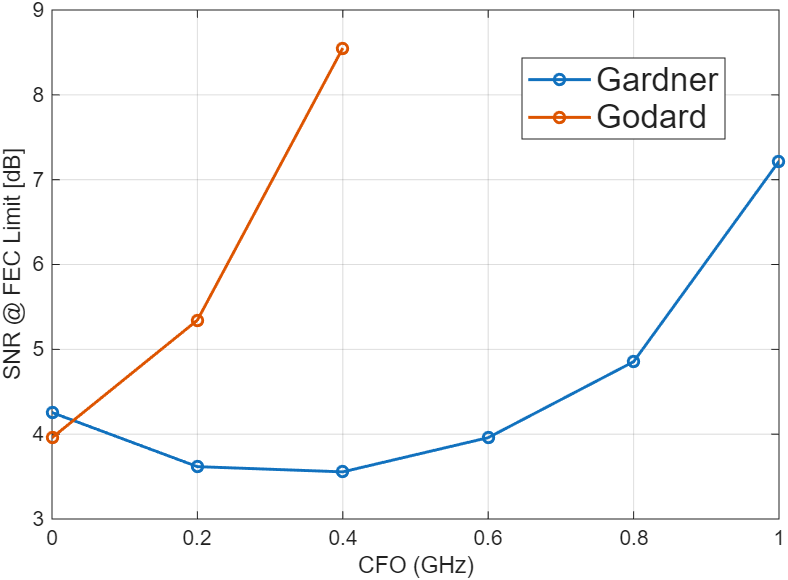
\includegraphics[width=0.6\textwidth]{max_cfo_combined_float.png}
    \caption{RSNR as CFO varies for each implementation. Points are omitted when the FEC limit is no longer reached at any SNR.}
    \label{fig:cfo_sweep_float}
\end{figure}

\paragraph{Correcting CFO} \Cref{fig:cfo_corrected_float} shows the RSNR for each implementation once the coarse CFO correction of \cref{sec:eqclk_methodology} is applied. The coarse estimate removes enough CFO for all implementations to achieve the FEC limit at the 3\,GHz tolerance. Godard and Gardner with the standard FFT/IFFT exhibit the same performance, but Godard performs better once the $2^k$ twiddle factors are included. Rounding the twiddle factors impacts both the FFT and IFFT; as Godard operates on data after the FFT, it is not affected by the additional loss of accuracy in the IFFT like Gardner.
\begin{figure}[H]
    \centering
    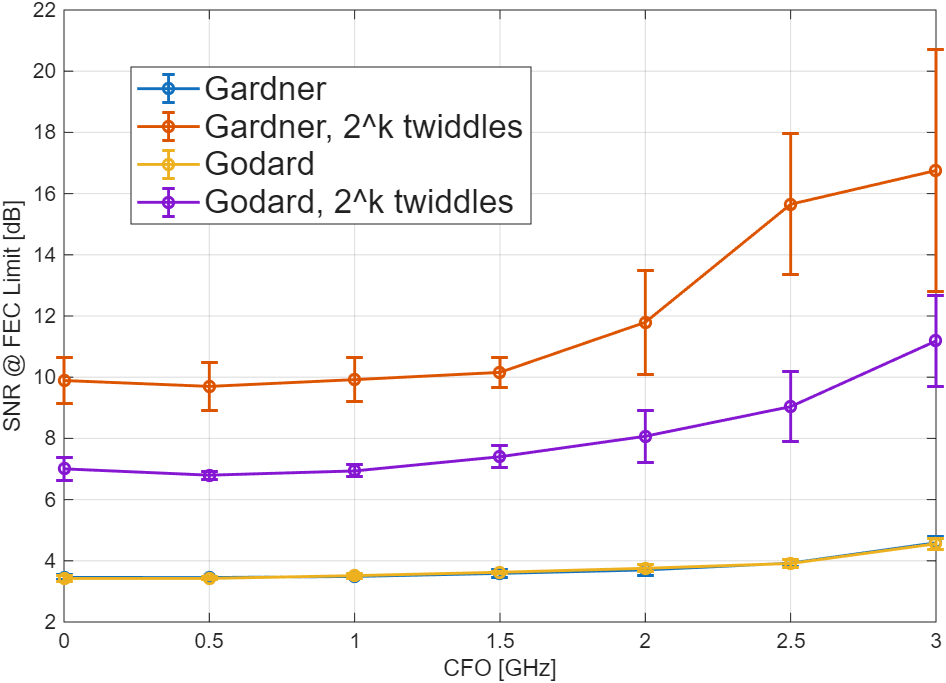
\includegraphics[width=0.6\textwidth]{cfo_sweep_corrected_float.png}
    \caption{RSNR as CFO varies with coarse CFO correction.}
    \label{fig:cfo_corrected_float}
\end{figure}

\subsection{Fixed-Point Precision}
So far implementations have been compared in floating-point arithmetic, avoiding the quantisation error present in a real coherent receiver. Each stage will have different precision requirements, so a search over precision combinations is required.

\paragraph{Adaptive equaliser.} \Cref{fig:aeq_fxp} shows how the precision of the adaptive equaliser gradient estimate impacts performance for each implementation while the static equaliser and clock recovery operate at high precision. Without $2^k$ twiddle factors the RSNR stays constant down to 4 bits until the FEC limit can no longer be reached at 2 bits. If $2^k$ twiddle factors are used then the compounding quantisation/rounding error limits to 6 bits before the RSNR rises, although the increase is small for Godard.
\begin{figure}[H]
    \centering
    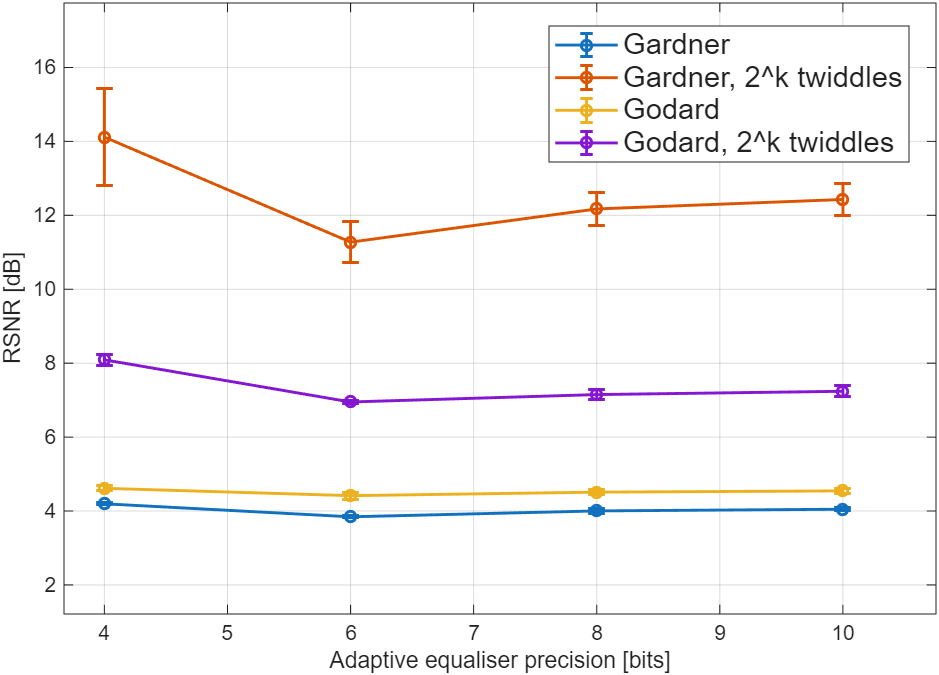
\includegraphics[width=0.65\textwidth]{aeq_fxp_sweep.png}
    \caption{RSNR as the fixed-point precision of adaptive equalisation varies, with static equalisation and clock recovery at high precision.}
    \label{fig:aeq_fxp}
\end{figure}

\paragraph{Static equaliser.} \Cref{fig:seq_fxp} shows the same precision sweep for the precision of the FFT/IFFT and the static filter when clock recovery and the adaptive equaliser are held at high precision. The precision requirement is slightly higher here but Godard and Gardner perform well down to 8 bits of precision. This can be explained by the FFT implementation: to avoid overflow each stage of the radix-2 FFT applies a 1/2 scaling with a bit-shift. For an FFT of size 128 this is 7 bit-shifts which at a precision lower than 8 bits means that the least significant bit is guaranteed to be lost at each stage, resulting in a very large quantisation error.
\begin{figure}[H]
    \centering
    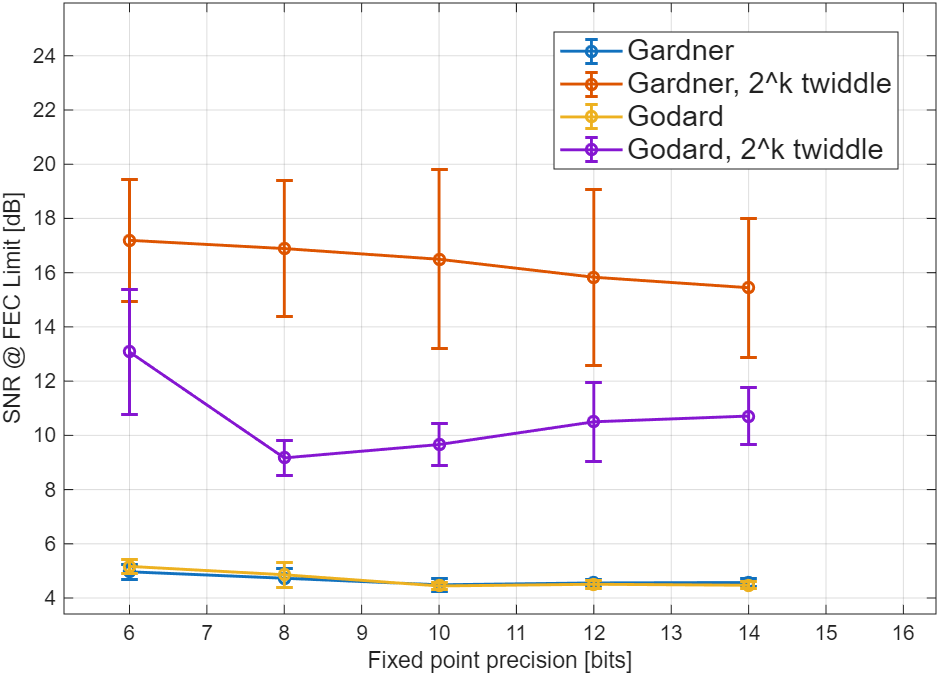
\includegraphics[width=0.65\textwidth]{seq_fxp_sweep.png}
    \caption{RSNR as the fixed-point precision of static equalisation varies, with adaptive equalisation and clock recovery at high precision.}
    \label{fig:seq_fxp}
\end{figure}

\paragraph{Clock recovery.} \Cref{fig:clk_fxp} shows the sweep for the precision of the timing error estimate and correction (Farrow interpolation or phase ramp). The loop filter is kept at high precision, as are the static and adaptive equalisers. Without the $2^k$ twiddle factors, Godard and Gardner perform the same down to 6 bits of precision before a sharp rise in RSNR at 4 bits, with Gardner failing to reach the FEC limit. Godard clearly outperforms Gardner when $2^k$ twiddle factors are used, as in the floating-point case. The Godard estimator is vulnerable to fixed point errors when computing the estimation metric from \cref{eq:godard_sum} as it requires a sum over $\beta N/\eta = 16$ terms where quantisation error can compound more than in the simple Gardner estimate of \cref{eq:gardner_ted}. However, Gardner is more susceptible to fixed-point precision at the correction stage where the Farrow interpolator performs many more cascaded operations than CORDIC.
\begin{figure}[H]
    \centering
    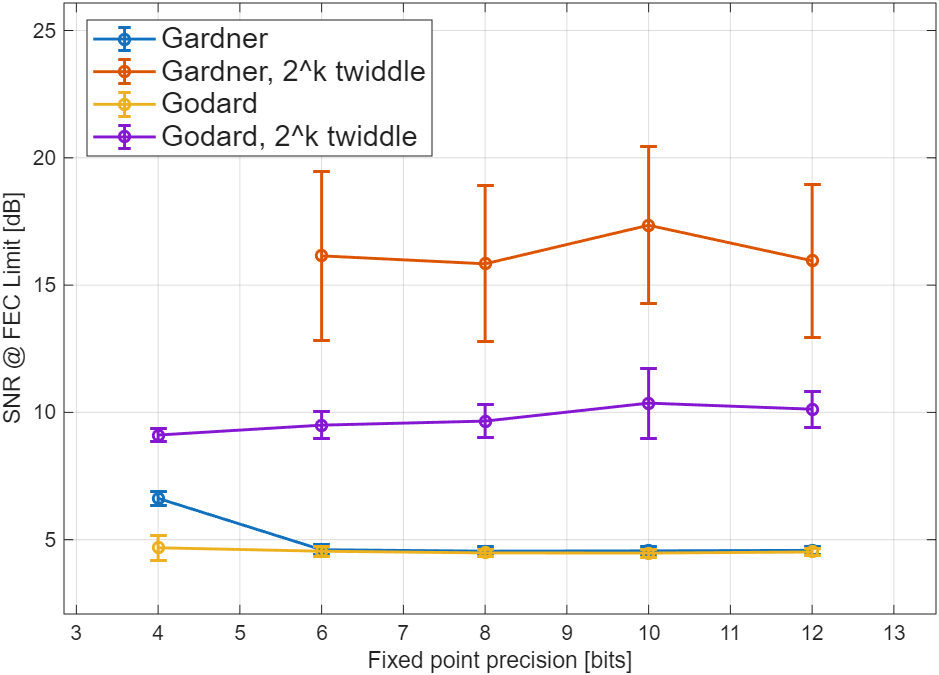
\includegraphics[width=0.65\textwidth]{clk_fxp_sweep.png}
    \caption{RSNR as the fixed-point precision of clock recovery varies, with static and adaptive equalisation at high precision.}
    \label{fig:clk_fxp}
\end{figure}

\paragraph{Low precision operating points.}
Combining each stage at low precision can introduce cascaded quantisation error which incurs an SNR penalty. \Cref{tab:clk_eq_fxp} shows the RSNR and energy breakdown of each algorithm at the lowest feasible precision combination taken from each individual sweep as well as a slightly higher precision combination for comparison. Godard consumes less energy than Gardner while performing similarly without $2^k$ twiddle factors and significantly outperforming it when $2^k$ twiddle factors are used. The choice of Godard implementation then depends on the balance of receiver energy and how the RSNR affects the transmitter energy. A suitable low-energy implementation is to use $2^k$ twiddle factors at the lowest precision combination, as higher precision only slightly reduces the RSNR. If a low RSNR is needed then foregoing the $2^k$ twiddle factors while still at the lowest precision is the most attractive as the higher precision only buys a small RSNR improvement. These two implementations will be taken forward to the full pipeline analysis in \cref{chapter:full_pipeline}.
\begin{table}[H]
    \centering
    \small
    \resizebox{\textwidth}{!}{%
    \begin{tabular}{llccccrrrr}
        \toprule
        \multirow{2}{*}{\textbf{Eq.}} & \multirow{2}{*}{\textbf{$2^k$}} & \multicolumn{3}{c}{\textbf{Precision (bits)}} & \multirow{2}{*}{\textbf{RSNR (dB)}} & \multicolumn{4}{c}{\textbf{Energy (pJ/bit)}} \\
        \cmidrule(lr){3-5} \cmidrule(lr){7-10}
        & & \textbf{Stat.} & \textbf{Adapt.} & \textbf{Clk} & & \textbf{$E_\mathrm{stat}$} & \textbf{$E_\mathrm{aeq}$} & \textbf{$E_\mathrm{clk}$} & \textbf{$E_\mathrm{tot}$} \\
        \midrule
        \multirow{2}{*}{Gardner} & \multirow{2}{*}{No}  & 8 & 4 & 6 & $4.85 \pm 0.07$  & 35.51 & 3.28 & 30.61 & 69.40 \\
                                 &                      & 10 & 6 & 8 & $3.99 \pm 0.07$  & 41.50 & 3.94 & 36.31 & 81.75 \\
        \midrule
        \multirow{2}{*}{Gardner} & \multirow{2}{*}{Yes} & 8 & 4 & 6 & $13.31 \pm 0.33$  & 6.19 & 3.28 & 30.61 & 40.07 \\
                                 &                      & 10 & 6 & 8 & $11.53 \pm 0.57$ &  7.08 & 3.94 & 36.31 & 47.33 \\
        \midrule
        \multirow{2}{*}{Godard}  & \multirow{2}{*}{No}  & 8 & 4 & 6 & $\mathbf{4.75 \pm 0.07}$  & 35.51 & 3.28 &  7.68 & \textbf{46.46} \\
                                 &                      & 10 & 6 & 8 & $4.34 \pm 0.07$  & 41.50 & 3.94 & 9.12 & 54.55 \\
        \midrule
        \multirow{2}{*}{Godard}  & \multirow{2}{*}{Yes} & 8 & 4 & 6 & $\mathbf{8.23 \pm 0.25}$ &  6.19 & 3.28 &  7.68 &  \textbf{17.14} \\
                                 &                      & 10 & 6 & 8 & $6.87 \pm 0.08$  &  7.08 & 3.94 &  9.12 & 20.13 \\
        \bottomrule
    \end{tabular}
    }
    \caption{Fixed-point performance and energy of the combined clock recovery and equalisation implementations at low- ($8/4/6$) and high-precision ($10/6/8$) operating points, with and without $2^k$ twiddle factors. The three precisions are those of the static equaliser, adaptive equaliser and clock recovery stages. Proposed candidates for an energy-efficient receiver are highlighted in bold.}
    \label{tab:clk_eq_fxp}
\end{table}

\paragraph{Oversampling rate.} These results assume an oversampling rate of 2. Modern coherent receivers can operate below 2 samples per symbol to reduce the load on analogue-to-digital converters (ADCs) and simplify the DSP \cite{Wang;24}. The Godard scheme allows the full equalisation and clock recovery block to operate at a fractional oversampling rate which reduces the number of operations per symbol. However, Gardner requires 2 samples per symbol so the output of the IFFT would need to be upsampled and the savings from a lower oversampling rate would be smaller.
% =====================================================================
\chapter{Carrier Recovery}\label{chapter:carrier_recovery}
% =====================================================================

\section{Introduction}

A coherent receiver recovers the transmitted symbols by mixing the incoming optical signal with a local oscillator (LO) laser, allowing the amplitude and phase of each symbol to be extracted directly. However, the transmitter and LO lasers generally have different centre frequencies and independent phase trajectories, producing a carrier frequency offset (CFO) and accumulated phase noise on the received symbols. Carrier recovery is the DSP stage responsible for estimating and removing these impairments before symbol decisions are made.

Carrier recovery is divided into two sequential stages. Frequency recovery performs a finer estimate of the CFO than that discussed in \cref{chapter:equalisation} and corrects it so that only slow residual phase variations remain. The frequency recovery discussed in this chapter is intended to be agnostic to whether the coarse CFO correction described there has already been applied, so as to generalise across receiver designs; the worst-case CFO of 3\,GHz is therefore assumed. Phase recovery then tracks and removes these residual phase errors on a block-by-block basis.

Two common carrier recovery algorithms, Rife \& Boorstyn and Viterbi \& Viterbi, are compared against low-complexity alternatives to quantify the trade-offs between energy consumption and performance in an energy-efficient carrier recovery block.

\section{Frequency Recovery}
\subsection{Carrier Frequency Offset}
A carrier frequency offset (CFO) occurs because the transmitter and local-oscillator lasers are free-running and never exactly aligned in centre frequency. The resulting beat appears as a linear phase ramp on the received samples. It is simulated by multiplying the signal by \(\exp(j\,2\pi\,\Delta f\, T_\mathrm{sym}\, k)\), where \(\Delta f\) is the frequency offset, \(T_\mathrm{sym} = 1/R_s\) the symbol period (carrier recovery operates at one sample per symbol), and \(k\) the symbol index.

\subsection{Isolating CFO}
All frequency recovery algorithms first require that the phase of the data be removed before estimation. For QPSK symbols \(c[i] = e^{j\left(\frac{\pi}{4} + m[i]\frac{\pi}{2}\right)}\), this can be done by raising each received symbol \(x[i] = c[i]e^{j(2\pi f_d i + \theta[i])} + n[i]\) to the fourth power to give
\begin{equation}
    z[i] = x^4[i] = e^{j(8\pi f_d i + 4 \theta[i])} + n'[i]
    \label{eq:blind_noise}
\end{equation}
where \(\theta\) is phase noise, \(f_d\) is the CFO, and \(n\) is additive noise. This allows all data symbols to be used in CFO estimation, but amplifies phase and additive noise, which degrades the estimation quality. The fourth power operation also requires three complex multiplications. An alternative is to use pilot symbols where the data phase is known beforehand, giving
\begin{equation}
    z[i] = x[i]c^*[i] = e^{j(2\pi f_d i + \theta[i])} + n[i],
    \label{eq:data_noise}
\end{equation}
which is more robust to noise and less computationally expensive. Some algorithms only require \(\arg(z[i])\), which is efficiently found using CORDIC as
\begin{equation}
    \arg(z[i]) = \{4\arg(x[i])\}|_{-\pi}^\pi
    \label{eq:phase_blind}
\end{equation}
for blind operation or
\begin{equation}
    \arg(z[i]) = \{\arg(x[i]) - \arg(c[i])\}|_{-\pi}^{\pi}
    \label{eq:phase_data}
\end{equation}
for data-aided operation, where the wrap operation can be done with no additional cost by aligning the wrap range to the overflow range of the fixed-point value used to store the phase.

\subsection{Rife \& Boorstyn}
The value of the CFO will appear as the strongest peak in the frequency spectrum of \(z[i], z[i+1], \dots, z[i+L]\) where \(L\) is the observation length. The Rife \& Boorstyn algorithm first performs an FFT on the observed sequence and finds the index \(k\) corresponding to the strongest peak. This coarse estimation is refined with a parabolic interpolation on the complex FFT values \(X_{k-1}, X_k, X_{k+1}\) to give \cite{Jacobsen2007}
\begin{equation}
    \delta = -\Re\left[\frac{X_{k+1} - X_{k-1}}{2X_k - X_{k-1} - X_{k+1}}\right].
    \label{eq:fft_refined}
\end{equation}
The updated index \(k' = k + \delta\) is then scaled by the sampling rate to find the true CFO. The resolution in \(k\) is \(\epsilon(k) = \frac{1}{2N_{FFT}}\). The CPON specification provides only \(L = 11\) training symbols, so data-aided operation without zero-padding gives \(\epsilon(\hat{f}_d) \approx 0.05\,R_s\), too coarse for the downstream phase recovery to correct. Zero-padding the training sequence to a larger \(N_{FFT}\) improves the resolution without requiring additional training data. The normalised mean-squared error (MSE) in the estimated CFO is shown in \cref{fig:fft_mcrb_data} for data-aided operation with 11 training symbols. A CFO estimate is computed for both polarisations and averaged to reduce the MSE. The modified Cramer-Rao bound (MCRB) provides a lower bound on the achievable MSE and is given by \cite{Andrea1994} (derived in \cref{appendix:mcrb})
\begin{equation}
    \mathrm{MCRB} = \frac{3}{2\pi^2 L^3 \times \mathrm{SNR}}.
\end{equation}
Rife \& Boorstyn achieves this bound above a threshold SNR of \(\approx 4\) dB, where the threshold SNR is defined as the SNR below which the estimator begins to deviate from the MCRB. Below this, noise contributes significantly to the FFT values and can lead to an incorrect index being chosen.
\begin{figure}[H]
    \centering
    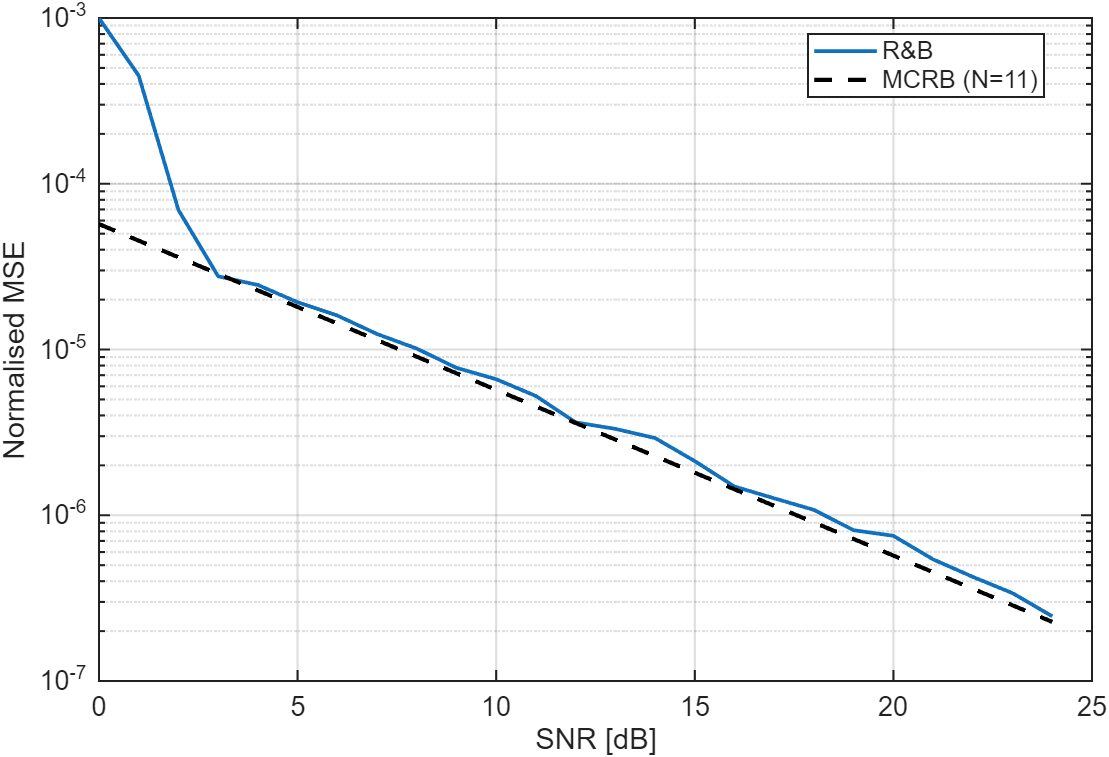
\includegraphics[width=0.65\textwidth]{MCRB_fft_data.png}
    \caption{Normalised MSE of the Rife \& Boorstyn algorithm with FFT size \(N_{FFT} = 512\) compared to the MCRB for \(L=11\) training symbols.}
    \label{fig:fft_mcrb_data}
\end{figure}
Data-aided operation is constrained by the length of the training sequence, but the accuracy of the Rife \& Boorstyn algorithm improves with longer observation lengths, as shown in \cref{fig:fft_mcrb_blind} for non-data-aided operation. The SNR threshold at which this algorithm begins to deviate from the MCRB is initially higher for non-data-aided operation, because the fourth-power operation amplifies noise, but it decreases for longer observation lengths.
\begin{figure}[H]
    \centering
    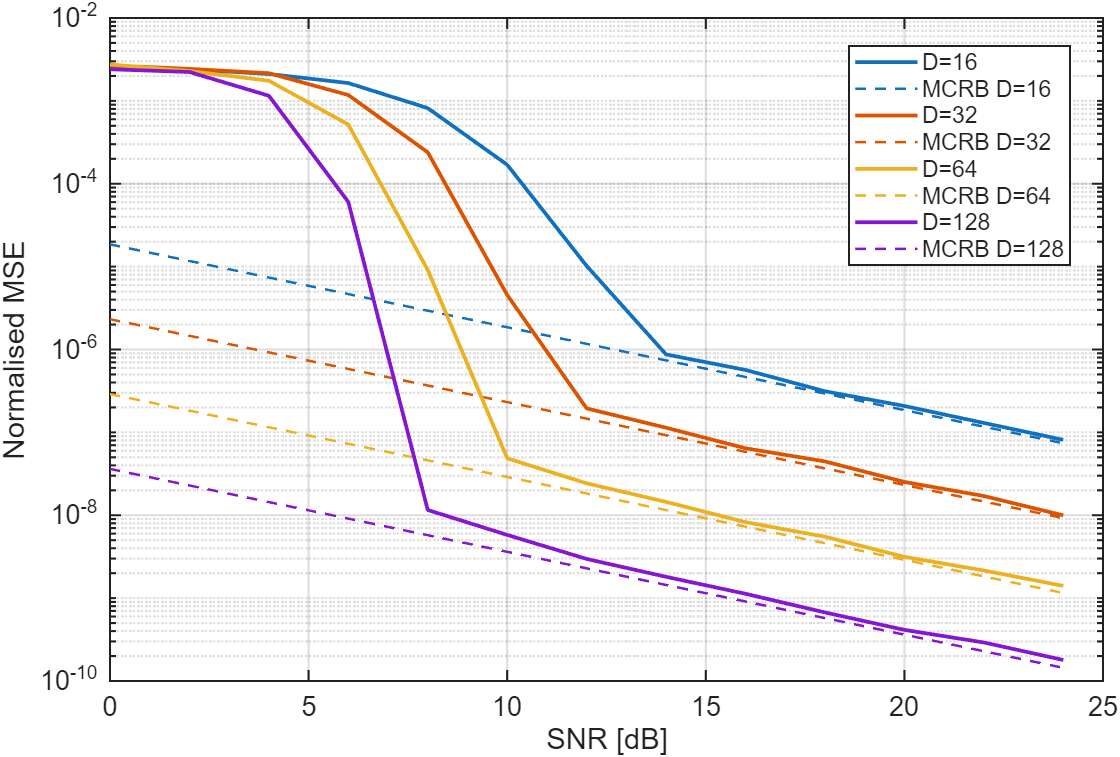
\includegraphics[width=0.65\textwidth]{MCRB_fft_blind.png}
    \caption{Normalised MSE of the Rife \& Boorstyn algorithm for non-data-aided operation and different observation lengths.}
    \label{fig:fft_mcrb_blind}
\end{figure}

\subsection{Differential Phase and Kay Estimator}
The Rife \& Boorstyn algorithm exhibits good performance even at low SNRs, but is computationally expensive. The FFT requires \(\frac{N_{FFT}}{2} \log_2(N_{FFT})\) complex multiplications and \(N_{FFT}\log_2(N_{FFT})\) complex additions. The fine search from \cref{eq:fft_refined} also requires a complex division. A cheaper approach would involve computing the phase difference
\begin{equation}
    \arg (z[i]) - \arg (z[i-1]) = 2 \pi f_d T_\mathrm{sym} + \theta[i] - \theta[i-1] + \eta[i]
    \label{eq:phase_diff}
\end{equation}
over several symbols and averaging to remove the effect of \(\theta\). Estimating \(f_d\) in this manner is vulnerable to the effect of additive noise on the phase \(\eta[i]\), so it exhibits poor accuracy. This can be improved with a second pass using the Kay estimator. The Kay estimator uses a least-squares approach, computing the estimated CFO as
\begin{equation}
    \hat{f}_d = \frac{R_s}{2 \pi} \sum_{k=1}^{L} \frac{6k(L-k)}{L(L^2 - 1)} \arg (z[k]z^*[k-1]).
\end{equation}
where \(\arg(z[k]z^*[k-1])\) computes the phase difference from \cref{eq:phase_diff} and \(\frac{6k(L-k)}{L(L^2 - 1)}\) is a weighting term that prioritises the contribution of phase differences in the middle of the observed sequence. This estimator is able to achieve the MCRB, but becomes biased at larger CFO and lower SNR as additive noise pushes the phase differences across the wrap boundary \cite{Morelli1998}. A first-pass coarse CFO correction is therefore applied before the Kay estimator to centre the residual phase differences away from this boundary.
The performance of the differential phase and Kay estimator for data-aided operation is shown in \cref{fig:diffkay_data}. The MCRB is achieved above a threshold SNR of \(\approx 7\) dB. This is higher than for Rife \& Boorstyn, but at a reduced computational cost. Unlike the Rife \& Boorstyn algorithm, the threshold SNR of the differential phase and Kay estimator does not depend on observation length, as shown in \cref{fig:diffkay_blind}.
\begin{figure}[H]
    \centering
    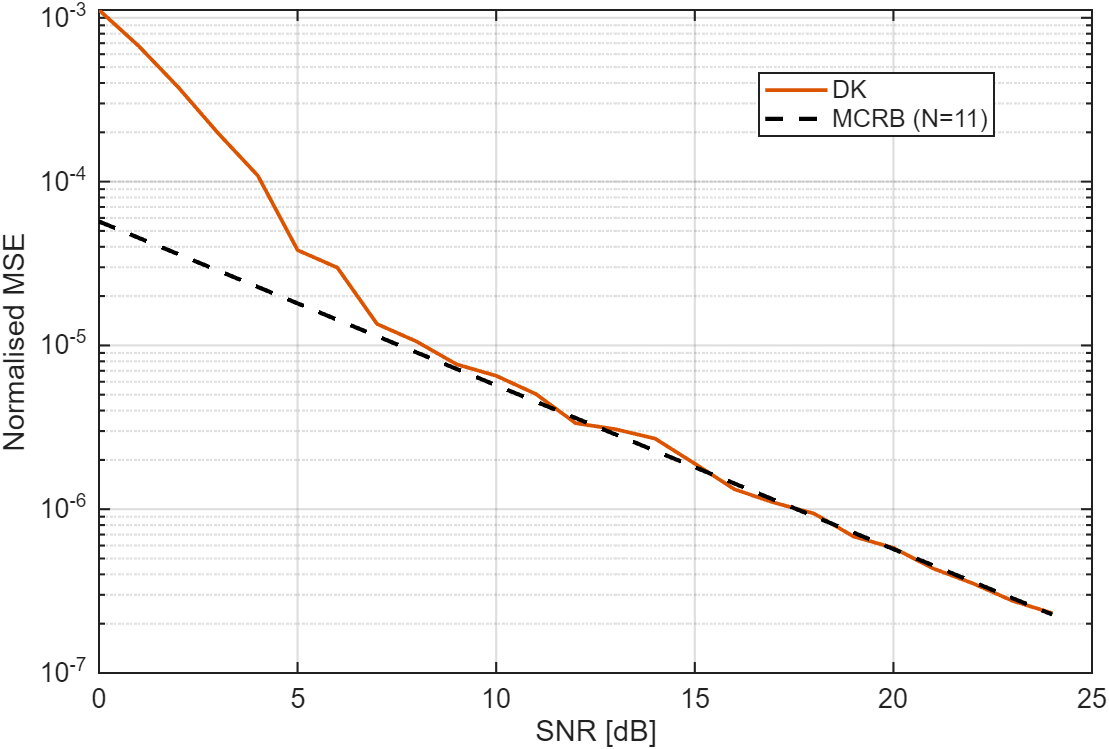
\includegraphics[width=0.65\textwidth]{MCRB_diffkay_data.png}
    \caption{Normalised MSE of frequency estimation with the differential phase and Kay estimator for \(L = 11\) training symbols.}
    \label{fig:diffkay_data}
\end{figure}

\begin{figure}[H]
    \centering
    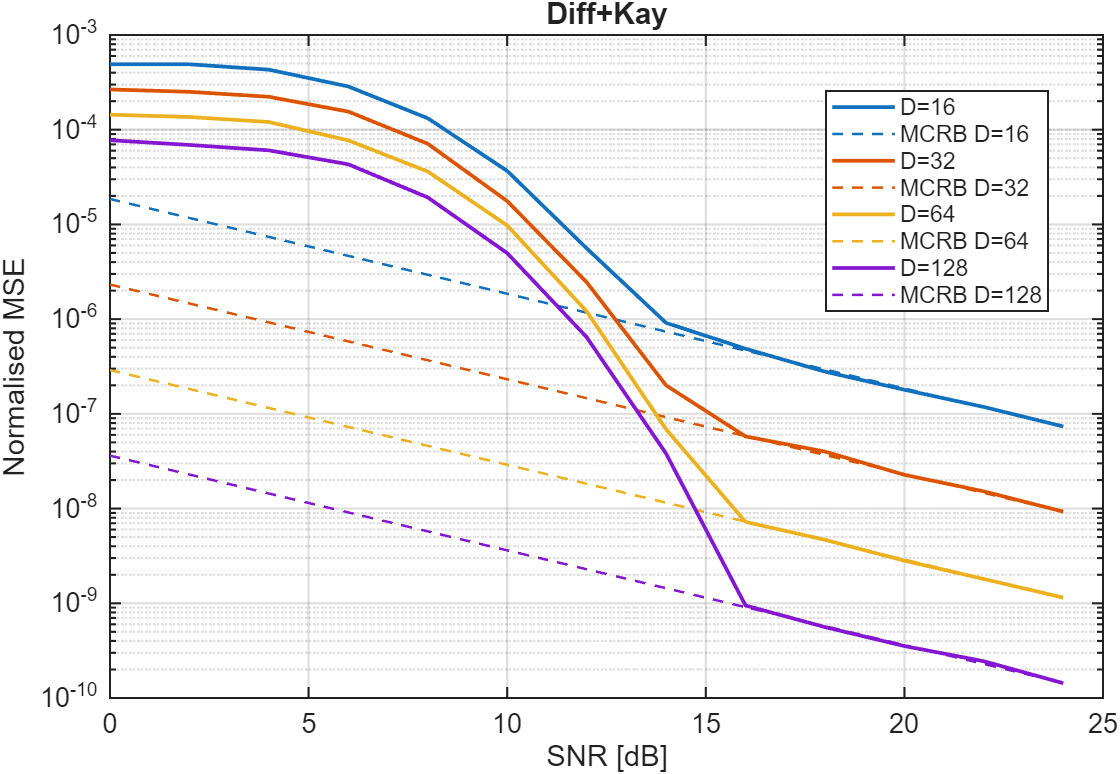
\includegraphics[width=0.65\textwidth]{MCRB_diffkay_blind.png}
    \caption{Normalised MSE of the differential phase and Kay estimator with blind operation for different observation lengths.}
    \label{fig:diffkay_blind}
\end{figure}
\subsection{Computational Complexity}
Here, the computational complexity of both frequency recovery algorithms is compared in terms of real multiplications and real additions. CORDIC is used to find phases and is assumed to cost the same as a real multiplication. The real division required by the Rife \& Boorstyn parabolic interpolation is assumed to cost the same as a multiplication since it is only performed once per estimate; a look-up-table reciprocal would meet this approximation at a small accuracy cost. All analysis applies to a single polarisation. If averaging is done over both polarisations, then all operations are doubled.
\paragraph{Rife \& Boorstyn}
The Rife \& Boorstyn algorithm requires an FFT followed by \(N_{FFT}\) comparisons of the magnitudes in the coarse search. Many of the FFT entries are 0 due to padding, which reduces the total number of operations needed. The interpolation requires the real part of a complex division
\begin{equation}
\Re \left[\frac{a + bj}{c + dj}\right] = \frac{ac + bd}{c^2 + d^2}.
\end{equation}
The total complexity is summarised in \cref{tab:fft_cost}; entries marked with a dagger ($^\dagger$) apply only to blind operation.
\begin{table}[H]
    \centering
    \begin{tabular}{lcc}
        \toprule
        Operation & RM & RA \\
        \midrule
        Forming \(z[i], \dots, z[i+L]\) & \(4L\), \(12L^\dagger\) & \(3L\), \(9L^\dagger\)\\
        FFT & \(2L \log_2(\frac{N_{FFT}}{L}) + 2N_{FFT}\log_2(L)\) & \(3L \log_2(\frac{N_{FFT}}{L}) + 3N_{FFT}\log_2(L)\)\\
        Search & \(2N_{FFT}\) & \(2N_{FFT}\)\\
        Interpolation & \(5\) & \(4\) \\
        \bottomrule
    \end{tabular}
    \caption{Computational complexity of estimating CFO with the Rife \& Boorstyn algorithm.}
    \label{tab:fft_cost}
\end{table}
\paragraph{Differential phase and Kay}
The differential phase and Kay estimator has lower complexity, only requiring CORDIC, real additions, and real multiplications. The fixed multiplications by the weights of the Kay estimator can be optimised into a low-energy shift-add circuit, but this is ignored for simplicity. The first-pass CFO correction involves forming the phase corrections of each training symbol as \(\phi[i] = \hat{f}_d\,i\), then applying them with CORDIC.
\begin{table}[H]
    \centering
    \begin{tabular}{lcc}
        \toprule
        Operation & RM & RA \\
        \midrule
        Forming \(\arg(z[i]), \dots, \arg(z[i+L])\) & \(2L\) & \(L\)\\
        Differential Phase & \(1\) & \(L-1\)\\
        First Pass Correction & \(2L\) & \(0\)\\
        Forming \(\arg(z[i]), \dots, \arg(z[i+L])\) & \(2L\) & \(L\) \\
        Kay & \(L\) & \(L-1\) \\
        \bottomrule
    \end{tabular}
    \caption{Computational complexity of estimating CFO with the differential phase and Kay estimator.}
    \label{tab:diffkay_cost}
\end{table}

\subsection{Optimising Bit Width}
These frequency recovery algorithms compute an estimate of the normalised CFO \(f_d / R_s\). For \(n\) bits of precision, the smallest normalised CFO that can be estimated is \(2^{-n}\) for an estimation range \(0 \leq |f_d / R_s| \leq 1\). In reality, a much smaller range of CFOs needs to be estimated. If the maximum permitted value of \(|f_d / R_s|\) is \(2^{-d}\), then \(d\) bits of precision that would otherwise be redundant can be reclaimed by scaling each estimate by \(2^d\) during calculation and inserting \(d\) bits into the final answer to recover the true normalised CFO. This improves the resolution to \(2^{-(n+d)}\) without any increase in energy consumption.

\subsection{Maximum CFO}
The theoretical limit on the maximum CFO that can be corrected is given by Nyquist as \(0.5\,R_s\). From \cref{eq:blind_noise}, we see that blind operation reduces this limit by a factor of 4. Both the Rife \& Boorstyn and differential phase and Kay estimators accurately estimate the CFO up to the Nyquist limit, as seen in \cref{fig:max_cfo}. Blind operation aliases as expected at \(f/R_s = 0.125\), making it viable for CFOs up to 3.8\,GHz at a symbol rate of 30.5\,GBd.
\begin{figure}[H]
    \centering
    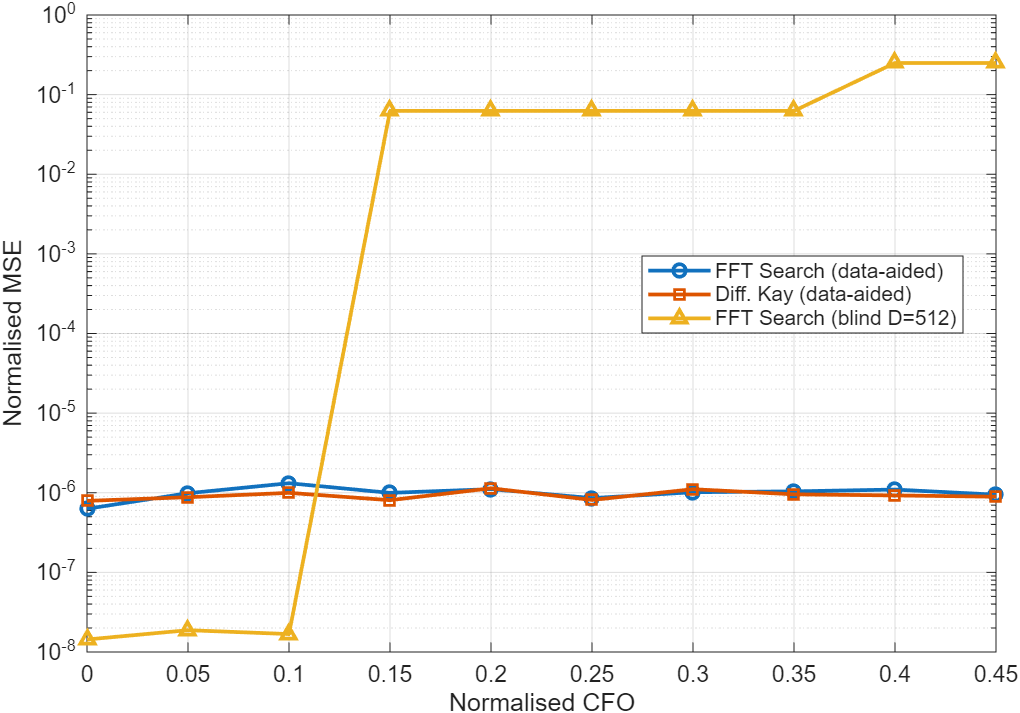
\includegraphics[width=0.65\textwidth]{max_cfo.png}
    \caption{Normalised MSE in CFO estimate (\(\mathrm{MSE}/R_s^2\)) vs.\ normalised CFO (\(f/R_s\)).}
    \label{fig:max_cfo}
\end{figure}

\section{Phase Recovery}
\subsection{Phase Noise}
Phase noise originates from the finite linewidth of the transmitter and LO lasers, whose phases follow a random walk. It is modelled as a Wiener process: independent Gaussian per-symbol phase increments with variance \(\sigma^2 = 2\pi\,\Delta\nu / R_s\), where \(\Delta\nu\) is the combined laser linewidth, are accumulated and applied as a multiplicative phase \(\exp(j\phi[k])\).

\subsection{Feed-Forward vs PLL Algorithms}
One of the first techniques investigated for phase recovery was a digital phase-locked loop (PLL) to incrementally correct the phase of each symbol with feedback, which simplifies phase estimation and correction through small-angle approximations. As with the equaliser (\cref{sec:aeq_parallel}), however, the symbol rate far exceeds the achievable CMOS clock speed, so symbols must be processed in blocks (here the 32-symbol CPON block), reducing the required clock speed to roughly 1\,GHz. Block processing hinders a PLL, as updates can only be made once per block, so feed-forward algorithms that operate on a whole block at once are used instead.

\subsection{Viterbi \& Viterbi}
The Viterbi \& Viterbi algorithm is well suited to QPSK and removes data phase with the fourth power operation of \cref{eq:blind_noise}. It then applies a maximum-likelihood filter \(w_{ML}[i]\) to estimate the phase error due to Wiener phase noise from the combined laser linewidth and any residual CFO as
\begin{equation}
    \hat{\theta}_{ML}[i] = \frac{1}{4} \arg\left(\sum_{k = 1}^{N} w_{ML}^*[k] z[k] \right) - \frac{\pi}{4}.
    \label{eq:viterbi_viterbi}
\end{equation}
A phase unwrapper is then applied before the phase error is corrected. This is readily adapted to block-based processing. If blocks of 32 symbols are used again, the ML filter can be applied to all symbols in the block and the estimated phase error applied to the entire block. This is only valid if the phase difference between the start and end of the block is small, meaning the laser linewidth cannot be too large and the preceding frequency recovery algorithm must correct most of the CFO. By increasing the time between phase estimates, block processing also increases the chance of cycle-slips in the phase unwrapper. The CPON specification provides one pilot symbol in every 32-symbol block that can be used to correct this \cite{Cheng2013PilotCycleSlip}. The correction estimates the number of \(\pi/2\) phase jumps \(n\) that occur between the unwrapped phase of a data symbol \(\hat{\theta}_\mathrm{PU}\) (the output of the phase unwrapper) and its corresponding pilot, then adjusts the unwrapped estimate as \(\hat{\theta}'_\mathrm{PU} = \hat{\theta}_\mathrm{PU} - n\frac{\pi}{2}\).
\subsection{Pilots-Only Correction}
While Viterbi \& Viterbi is commonly used for QPSK, a simpler approach is to compute the phase error from the pilot symbol using \cref{eq:data_noise} and apply this to the whole block. This also relies on a small phase change across the block and is more vulnerable to additive noise. However, QPSK allows for \(\pm \pi/4\) error in the phase estimate before an incorrect decision is made, which makes it robust to the drop in accuracy associated with this approach.

\subsection{Computational Complexity}
\paragraph{Viterbi \& Viterbi}
For a block-based approach, the length of the filter will be the block length. Phases are again found with CORDIC. The cost of the phase estimate for each block is shown in \cref{tab:viterbi_cost}.
\begin{table}[H]
    \centering
    \begin{tabular}{lcc}
        \toprule
        Operation & RM & RA \\
        \midrule
        Forming \(z[i], \dots, z[i+N]\) & \(12N\) & \(9N\)\\
        Computing \(\hat{\theta}_{ML}\) & \(4N+1\) & \(3N+2(N-1)+1\)\\
        \bottomrule
    \end{tabular}
    \caption{Computational complexity of block-based Viterbi \& Viterbi.}
    \label{tab:viterbi_cost}
\end{table}
\paragraph{Pilots-Only}
Only phases are needed, so the entire estimation can be performed with CORDIC. The pilot phase is also known beforehand, so does not contribute to the computational cost. The total cost of the phase estimate is shown in \cref{tab:pilot_cost}.
\begin{table}[H]
    \centering
    \begin{tabular}{lcc}
        \toprule
        Operation & RM & RA \\
        \midrule
        Forming \(\arg(z[i]) = \hat{\theta}\) & \(1\) & \(1\)\\
        \bottomrule
    \end{tabular}
    \caption{Computational complexity of Pilots-Only correction.}
    \label{tab:pilot_cost}
\end{table}

\section{Methodology}

\paragraph{Phase recovery comparison.} The two phase recovery algorithms are compared in isolation by simulating an AWGN channel with Wiener phase noise. BER is estimated by Monte Carlo simulation over 10 independent realisations for each combination of laser linewidth and SNR.

\paragraph{Frequency recovery comparison.} Three frequency recovery configurations are compared by the receiver effort needed to estimate the CFO accurately enough for the downstream phase recovery: data-aided differential phase and Kay, blind Rife \& Boorstyn with \(D = N_{FFT} = 2048\) (the largest power-of-two FFT that fits within a 3712-symbol subframe), and data-aided Rife \& Boorstyn with \(N_{FFT} = 2048\). The channel applies a CFO drawn at random with 1\,MHz Wiener phase noise and AWGN at 20\,dB. Each algorithm produces one CFO estimate per subframe; the per-subframe estimates are averaged and the RMS error over 10 random CFO/noise realisations is recorded as a function of the number of averaged subframes \(N\). For each algorithm the smallest \(N\) reaching two targets is found: the \(\approx 10\)\,MHz residual the phase recovery can absorb (consistent with its linewidth tolerance in \cref{fig:vv_vs_pilots}) and the tighter 1\,MHz phase-noise floor. A high fixed-point precision (32-bit word length, 16 fractional bits) is used so that quantisation is not the limiting factor, and all angle estimates and rotations are performed with CORDIC.

\paragraph{Operation counts.} The receiver effort of each algorithm is reported as the per-subframe real-multiplication (RM) and real-addition (RA) counts of \cref{tab:fft_cost,tab:diffkay_cost}, evaluated for the observation lengths above and multiplied by the number of subframes \(N\) required to reach each target.

\paragraph{Fixed-point precision.} The selected chain, data-aided differential phase and Kay frequency recovery followed by pilots-only phase recovery, is then characterised in fixed point. Precision refers to the number of fractional bits carried in each calculation; the word length is this precision plus a fixed integer part sized to the dynamic range of the quantity. The CFO is normalised to the maximum tolerance so all calculations are contained within [-1,1] while any angles require 3 integer bits to represent $[-\pi, \pi]$ which are included in the total energy consumption of operations. The two stages are swept independently: the phase-recovery precision is swept with the frequency estimate held at high precision, then the frequency-recovery precision is swept with the phase estimate held high. Every fixed-point operation in the swept stage uses that fractional precision, including the CORDIC angle estimates and rotations, whose iteration count is set equal to the precision, and the frequency estimator's phase and accumulator datapaths. The channel applies a 3\,GHz CFO with 1\,MHz Wiener phase noise, and the frequency estimate is averaged over 12 subframes (the 10\,MHz operating point of \cref{tab:fr_subframe}) before correction. For each precision the pre-FEC BER is found by Monte Carlo over the SNR sweep, and the RSNR is reported as a mean with standard deviation.

\paragraph{Carrier-recovery energy.} At selected precision pairs the receiver energy per bit is evaluated with the arithmetic model of \cref{sec:rx_energy}, each operation taken at the fractional precision of the stage that produces it. The differential-Kay estimate cost (\cref{tab:diffkay_cost}) is amortised over one 3712-symbol subframe; the pilots-only estimate cost (\cref{tab:pilot_cost}) is amortised over one 32-symbol block; and the combined CFO and phase rotation applied to every symbol is charged as a single real multiplication per symbol at the phase-recovery precision.

\section{Results \& Discussion}
\subsection{Phase Recovery Performance}
To replace Viterbi \& Viterbi with the simplified pilots-only phase correction, it must exhibit comparable performance over the range of linewidths that could be expected during operation of the network. The BER for each phase recovery algorithm as SNR varies is shown in \cref{fig:vv_vs_pilots}. Both algorithms have almost identical performance (plots overlapping) and are reliable up to 10\,MHz, well beyond the 1\,MHz maximum given in the CPON spec. As they perform almost identically over the full linewidth and SNR range, the simpler pilots-only correction is adopted for phase recovery.
\begin{figure}[H]
    \centering
    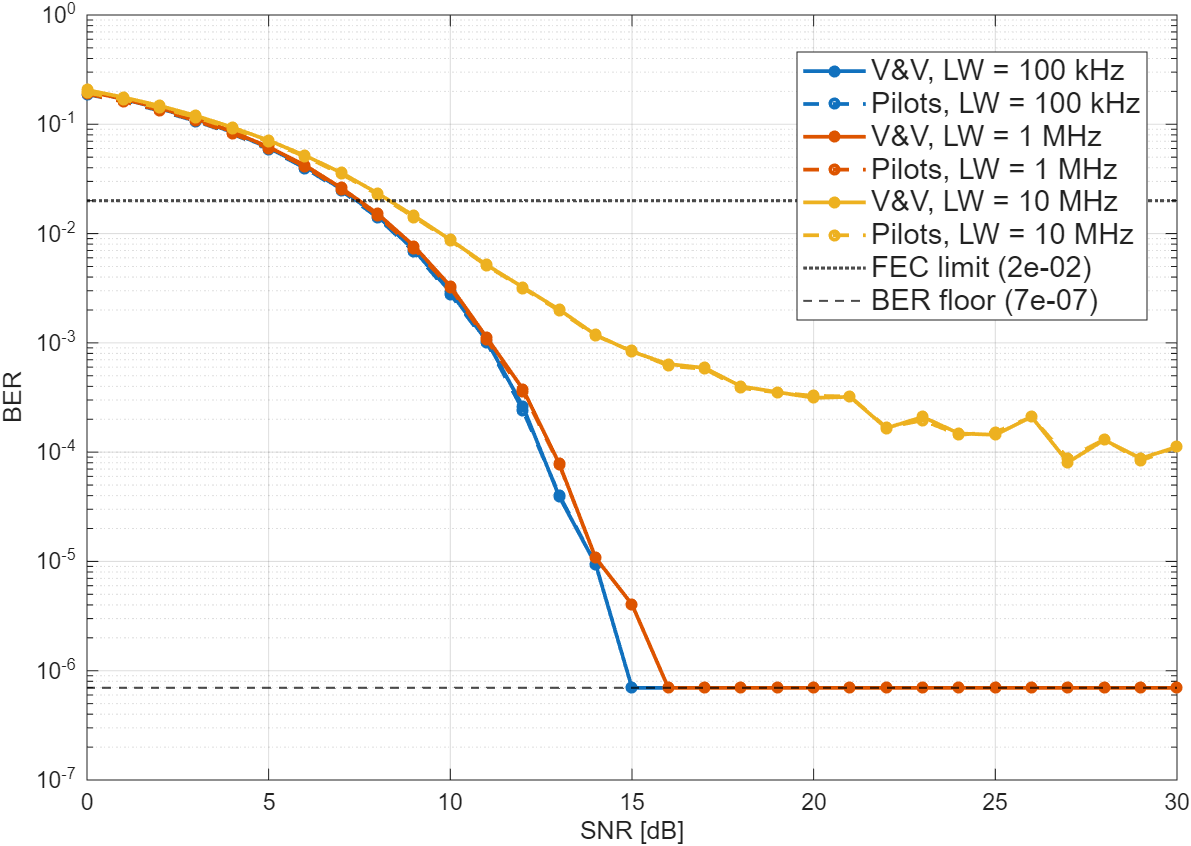
\includegraphics[width=0.65\textwidth]{vv_vs_pilots.png}
    \caption{Performance comparison of V\&V and Pilots-Only phase correction.}
    \label{fig:vv_vs_pilots}
\end{figure}

\subsection{Frequency Recovery: Subframe Averaging}
The data-aided algorithms form their CFO estimate from only the 11 CPON training symbols, so a single-subframe estimate is noisy. The estimate can be refined by averaging over several subframes, provided the CFO stays constant over that interval, but this multiplies the receiver effort. \Cref{tab:fr_subframe} reports, for each algorithm, the number of subframes \(N\) that must be averaged to reduce the CFO enough to allow phase recovery to correct the remaining error. Ideally this should be $\approx 1$\,MHz, the same as the phase noise, but from \cref{fig:vv_vs_pilots} it seems that 10\,MHz does not incur a significant RSNR penalty so should also be considered.

\Cref{fig:subframe_averaging} compares how the CFO estimation error decreases as more subframes are averaged over for each of the frequency recovery algorithms. The largest FFT size contained within one subframe is 2048, which is used for both Rife \& Boorstyn estimators. Blind Rife \& Boorstyn achieves the 10\,MHz error in one subframe but takes $\approx 10$ subframes to reliably be below 1\,MHz error. The differential phase and Kay estimator takes $\approx 12$ subframes to achieve 10\,MHz error but settles on 1\,MHz error at $\approx 300$ subframes. Data-aided Rife \& Boorstyn levels off at $\approx 16$\,MHz error which suggests that reusing the same training symbol sequence each time biases the estimator. \Cref{tab:fr_subframe} compares the number of operations needed to achieve the CFO error limits. The differential phase and Kay estimator is the clear choice if a residual CFO of 10\,MHz is acceptable as the operation count is far lower than blind Rife \& Boorstyn and 12 subframes should be a short enough window for the CFO to be constant over. At 1\,MHz the computational burden of the differential phase and Kay estimator increases significantly, although still lower than blind Rife \& Boorstyn which is prohibitively expensive, and averaging over 300 subframes increases the risk of the CFO varying and invalidating the average. Thus an energy-efficient receiver should employ the differential phase and Kay estimator with a target of 10\,MHz error.
\begin{figure}[H]
    \centering
    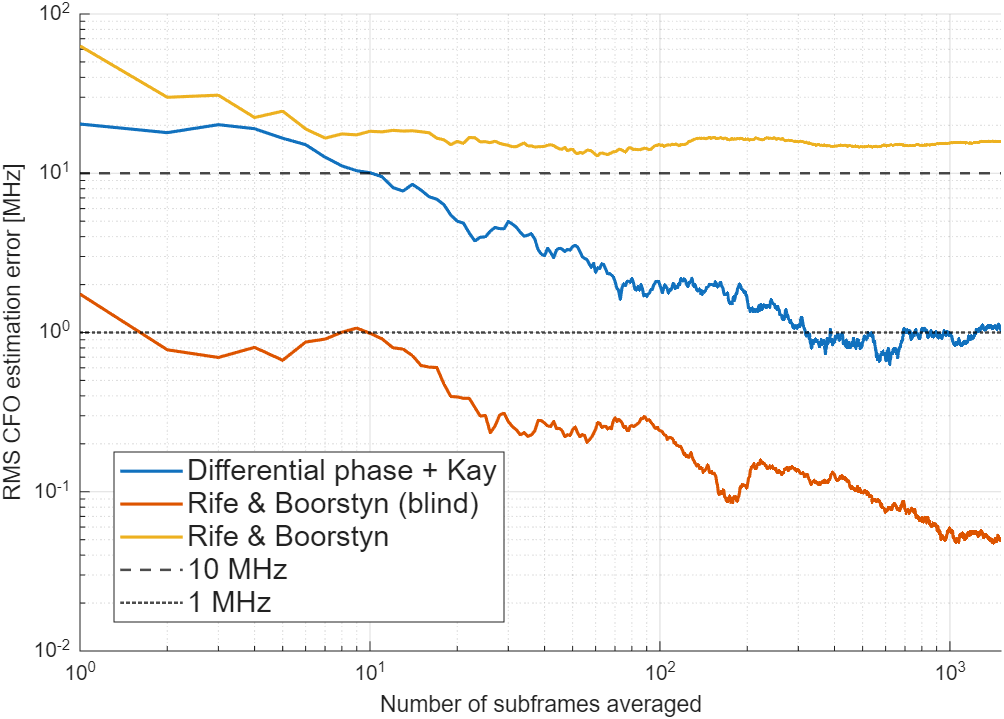
\includegraphics[width=0.65\textwidth]{subframe_averaging.png}
    \caption{CFO estimation error vs number of averaged subframes for each frequency recovery algorithm at high precision.}
    \label{fig:subframe_averaging}
\end{figure}
\begin{table}[H]
    \centering
    \small
    \begin{tabular}{@{}p{4.7cm} c c rr rr@{}}
        \toprule
        & & & \multicolumn{2}{c}{Per subframe} & \multicolumn{2}{c}{Total} \\
        \cmidrule(lr){4-5}\cmidrule(lr){6-7}
        FR algorithm & Target & \(N\) & RM & RA & RM & RA \\
        \midrule
        Differential phase and Kay      & 10\,MHz & 12   & 78 & 42 & 936      & 504 \\
        (data-aided, \(L=11\))          & 1\,MHz  & 300 &    &    & 23\,400 & 12\,600 \\
        \midrule
        Rife \& Boorstyn                & 10\,MHz & 1    & 73\,733 & 90\,116 & 73\,733  & 90\,116 \\
        (blind, \(D=N_{FFT}=2048\))     & 1\,MHz  & 10    &         &         & 737\,330 & 901\,160 \\
        \bottomrule
    \end{tabular}
    \caption{Subframes to average (\(N\)) and resulting operation counts (real multiplications RM, real additions RA) to reach a 10\,MHz and a 1\,MHz RMS CFO estimate. The per-subframe counts are target-independent. Data-aided Rife \& Boorstyn reaches neither target (its error floors at 17\,MHz).}
    \label{tab:fr_subframe}
\end{table}
\subsection{Fixed Point}
The most energy-efficient implementation of the differential phase and Kay estimator combined with pilot-based phase correction must select fixed-point values that balance energy consumption with RSNR. \Cref{fig:dk_precision} shows the impact of the precision of both frequency and phase recovery estimates on RSNR with a CFO of 3\,GHz and a linewidth of 1\,MHz. The differential phase and Kay estimator performs well down to 10 bits of precision before failing. This seems high but is a consequence of the CFO range that the estimator must track. If this stage should correct up to 3\,GHz, then even with the bit-width optimisation mentioned previously the estimator requires $\left\lceil\log_2(3000/10)\right\rceil = 9$ bits to give a resolution of 10 MHz. If the coarse CFO correction of \cref{chapter:equalisation} was included in the analysis then the required range for this stage to track could be reduced and fewer bits would be needed. The pilots-only phase estimate can operate at much lower precision, with no change in performance down to 6 bits and only a small increase in RSNR at 4 bits. This gives a resolution of 1/16 radians in the phase which is $\approx 8\,\%$ of the $\pi/4$ phase error tolerance of QPSK.
\begin{figure}[H]
    \centering
    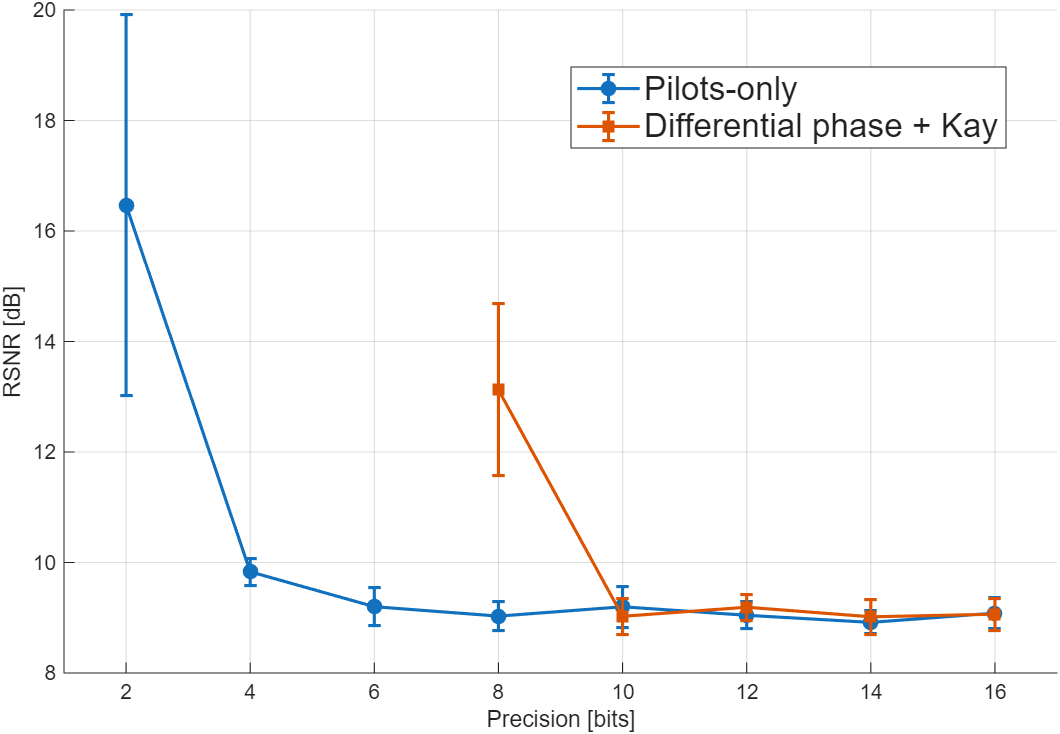
\includegraphics[width=0.65\textwidth]{dk_precision.png}
    \caption{RSNR vs CFO estimation precision of the differential phase and Kay estimator when phase correction is held at high precision.}
    \label{fig:dk_precision}
\end{figure}



\paragraph{Low precision operating point.} As in \cref{chapter:equalisation} we now infer a suitable low-precision operating point from \cref{fig:dk_precision}. The lowest precision combination is 4 bits for the phase error estimate and 10 bits for the CFO estimate; 6 and 12 bits are also considered to absorb any cascaded quantisation error. Amortisation of the estimates means that the phase correction dominates the energy consumption. Carrier recovery consumes energy on the order of fJ/bit, much less than equalisation or clock recovery which is on the order of pJ/bit.
\begin{table}[H]
    \centering
    \small
    \begin{tabular}{ccccccc}
        \toprule
        CFO precision (bits) & Phase error precision (bits) & RSNR (dB) & $E_\mathrm{fr}$ & $E_\mathrm{pr}$ & $E_\mathrm{apply}$ & $E_\mathrm{total}$ \\
        \midrule
        10 & 4 & $10.09\pm0.48$ & 1.68 & 0.48 & 12.12 & 14.28 \\
        12 & 6 & $9.14\pm0.38$ & 2.39 & 1.00 & 27.27 & 30.66 \\
        \bottomrule
    \end{tabular}
    \caption{RSNR and energy (fJ/bit) of the CFO estimate ($E_\mathrm{fr}$), phase error estimate ($E_\mathrm{pr})$, and the CORDIC rotation to apply both corrections.}
    \label{tab:cr_cost}
\end{table}




\chapter{Full DSP Pipeline}\label{chapter:full_pipeline}
\section{Introduction}
The preceding chapters characterised each DSP block in isolation. This chapter assembles them into a complete fixed-point receiver and compares the end-to-end performance and energy of candidate implementations. It first describes the remaining front-end blocks (the ADC, and the orthogonalisation and deskew that correct front-end imperfections), then defines the operating points carried forward from the equalisation, clock recovery, and carrier recovery chapters and compares their required SNR and energy, before combining the receiver and transmitter contributions into a single system energy comparison.

\section{Analogue-Digital Converters (ADCs)}
The optical front end mixes the received signal with the LO in a pair of $90\degree$ hybrids and balanced photodetectors, producing four baseband photocurrents: the in-phase and quadrature components of each polarisation. A bank of ADCs digitises these waveforms before any digital processing. The resolution of these ADCs sets the quantisation-noise floor for the subsequent DSP, while their conversion energy is a major component of the receiver front-end budget.

\paragraph{Quantisation-error SNR.}
A uniform quantiser of $B$ bits spanning a full-scale range $V_\mathrm{FS}$ has a step size $\Delta = V_\mathrm{FS}/2^B$. The quantisation error $e$ can be modelled as uniformly distributed over $[-\Delta/2,\,\Delta/2]$ with variance
\begin{equation}
    \sigma_e^2 = \frac{1}{\Delta}\int_{-\Delta/2}^{\Delta/2} e^2\,\mathrm{d}e = \frac{\Delta^2}{12}.
    \label{eq:quant_var}
\end{equation}
For a full-scale sinusoid of amplitude $V_\mathrm{FS}/2$ the signal power is $V_\mathrm{FS}^2/8$, so the signal-to-quantisation-noise ratio is
\begin{equation}
    \mathrm{SQNR} = \frac{V_\mathrm{FS}^2/8}{\Delta^2/12} = \frac{V_\mathrm{FS}^2/8}{V_\mathrm{FS}^2/(12\cdot 2^{2B})} = \frac{3}{2}\,2^{2B},
\end{equation}
or, in decibels,
\begin{equation}
    \mathrm{SQNR_{dB}} = 6.02\,B + 1.76.
    \label{eq:sqnr}
\end{equation}
A real ADC introduces its own noise and distortion which limits the achievable resolution. Including the SNR from these distortions in \cref{eq:sqnr} gives the effective number of bits, the number of bits in an equivalent ideal ADC, as
\begin{equation}
    \mathrm{ENOB} = \frac{\mathrm{SNDR_\mathrm{dB}}-1.76}{6.02}.
\end{equation}
where $\mathrm{SNDR_{dB}}$ is the total SNR from quantisation and distortions in decibels. The energy per sample for a range of ADCs is shown in \cref{fig:adc}. A floor of $\approx 1$ pJ/sample is observed for an SNDR lower than 60 dB, corresponding to an ENOB of 9.6. This is higher than the precisions used so far in the DSP blocks, so we take 1\,pJ/sample as the ADC's flat energy cost and use an ENOB of 6 in the following analysis. Each QPSK symbol is digitised as an in-phase and a quadrature sample, two conversions carrying two bits in total, so 1\,pJ/sample corresponds to an ADC energy of 1\,pJ/bit.
\begin{figure}[H]
    \centering
    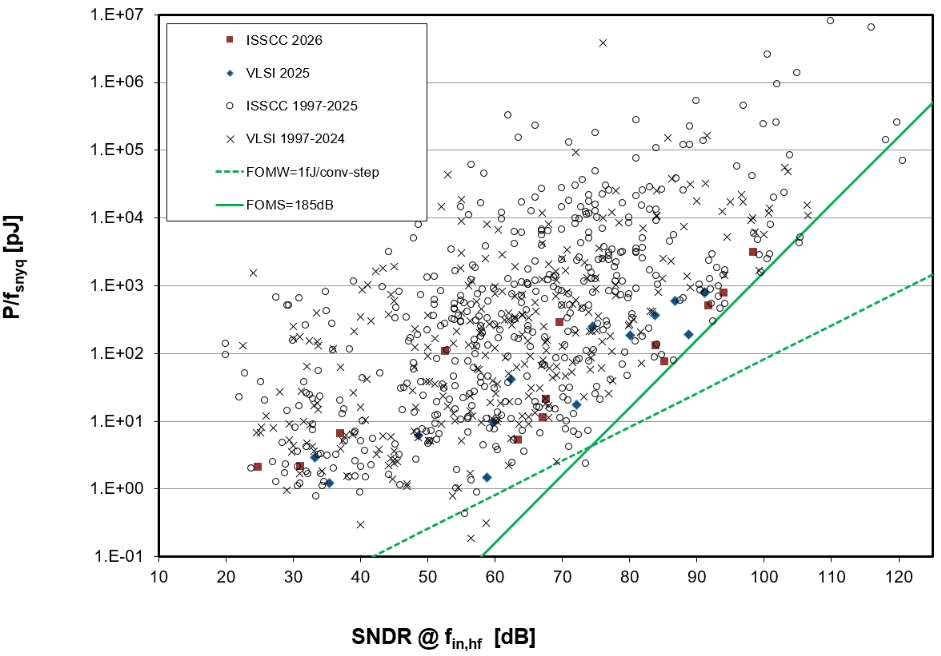
\includegraphics[width=0.8\textwidth]{adc.jpeg}
    \caption{ADC energy per bit (pJ) as SNDR (dB) varies \cite{adc_survey}.}
    \label{fig:adc}
\end{figure}
\section{Orthogonalisation and Deskew}
In practice the optical hybrid and the electrical paths feeding the ADCs are imperfect, leaving the in-phase and quadrature components mismatched. A quadrature error arises when the hybrid's phase shift departs from $90\degree$, so that the I and Q axes are no longer orthogonal. A separate I/Q timing skew arises from unequal propagation delays in the two paths, so that the I and Q samples are taken at slightly different instants.

Quadrature errors are removed by orthogonalisation, usually the Gram--Schmidt orthogonalisation procedure (GSOP) \cite{Mello;21,coherent_receivers}, which rescales the two components to equal power and subtracts the correlated part of one from the other to restore orthogonality. The timing skew is corrected by fractional-delay interpolation that realigns the I and Q sampling instants.

\subsection{Orthogonalisation}
Let $r_I[k]$ and $r_Q[k]$ be the in-phase and quadrature samples of one polarisation. GSOP first normalises the in-phase component to unit power,
\begin{equation}
    I_\mathrm{out}[k] = \frac{r_I[k]}{\sqrt{P_I}}, \qquad P_I = \mathbb{E}\!\left[r_I^2\right].
    \label{eq:gsop_i}
\end{equation}
The part of $r_Q$ correlated with $r_I$ is then subtracted and the residual normalised to unit power,
\begin{equation}
    Q'[k] = r_Q[k] - \frac{\rho_{IQ}}{P_I}\,r_I[k], \qquad
    Q_\mathrm{out}[k] = \frac{Q'[k]}{\sqrt{P_Q}},
    \label{eq:gsop_q}
\end{equation}
where $\rho_{IQ} = \mathbb{E}\!\left[r_I r_Q\right]$ is the I/Q correlation and $P_Q = \mathbb{E}\!\left[Q'^2\right]$ the residual power. The resulting $I_\mathrm{out}$ and $Q_\mathrm{out}$ are orthogonal and of equal power.

The statistics $P_I$, $\rho_{IQ}$ and $P_Q$ are estimated by averaging over a block of samples and, like the carrier frequency offset, vary far more slowly than the symbol rate; they are therefore computed once per block and reused, amortising their cost to a negligible per-symbol contribution. Folding the normalisation constants into the decorrelation coefficient, \cref{eq:gsop_i,eq:gsop_q} reduce to
\begin{equation}
    I_\mathrm{out}[k] = a\,r_I[k], \qquad Q_\mathrm{out}[k] = b\,r_Q[k] + c\,r_I[k],
\end{equation}
with the precomputed constants $a = 1/\sqrt{P_I}$, $b = 1/\sqrt{P_Q}$ and $c = -\rho_{IQ}/(P_I\sqrt{P_Q})$. Each output sample then costs $3$ real multiplications and $1$ real addition; running on the oversampled signal scales this by $\eta$, giving the per-symbol counts in \cref{tab:gsop_cost}.

\begin{table}[H]
    \centering
    \begin{tabular}{lcc}
        \toprule
        Stage & RM / symbol & RA / symbol \\
        \midrule
        GSOP application & $3\eta$ & $\eta$ \\
        \bottomrule
    \end{tabular}
    \caption{Per-symbol real multiplication (RM) and real addition (RA) counts for the Gram--Schmidt orthogonalisation, per polarisation. $\eta$ is the receiver oversampling factor. The block statistics $P_I$, $\rho_{IQ}$ and $P_Q$ are estimated infrequently and reused, contributing negligibly per symbol.}
    \label{tab:gsop_cost}
\end{table}

\subsection{Deskew}
The skew is compensated by a Lagrange fractional-delay interpolator of order $N$, implemented as a FIR filter of $N_\mathrm{DS} = N+1$ taps applied independently to each real I and Q component \cite{Mello;21}. The filter coefficients depend only on the (static) per-component delays, so the Lagrange weight computation is performed once at configuration time and amortised to zero per symbol. Each output sample of a real $N_\mathrm{DS}$-tap FIR therefore costs $N_\mathrm{DS}$ real multiplications and $N_\mathrm{DS}-1$ real additions. Per polarisation the in-phase and quadrature components are filtered separately, giving two real FIRs, and the filters run on the oversampled signal so their counts scale by the oversampling factor $\eta$. The resulting per-symbol costs are given in \cref{tab:deskew_cost}.

\begin{table}[H]
    \centering
    \begin{tabular}{lcc}
        \toprule
        Stage & RM / symbol & RA / symbol \\
        \midrule
        Deskew FIRs (2 real FIRs $\times$ $N_\mathrm{DS}$ taps) & $2\eta N_\mathrm{DS}$ & $2\eta(N_\mathrm{DS}-1)$ \\
        \bottomrule
    \end{tabular}
    \caption{Per-symbol real multiplication (RM) and real addition (RA) counts for the deskew interpolator, per polarisation. $N_\mathrm{DS} = N+1$ is the FIR length for a Lagrange interpolator of order $N$, and $\eta$ the receiver oversampling factor. The Lagrange coefficients are precomputed from the static skew and so do not contribute to the per-symbol count.}
    \label{tab:deskew_cost}
\end{table}

\section{Methodology}
The complete receiver is simulated in fixed point and scored on the same channel and figures of merit used for the individual blocks, so that the operating points selected in the earlier chapters can be evaluated end to end.

\paragraph{Channel and transmitter.} Each trial generates whole CPON downstream subframes using the framing of \cref{chapter:cpon} (3712 symbols per subframe, with 11 training symbols and one pilot in every 32-symbol block), five subframes per trial. The DP-QPSK signal is RRC-shaped ($\beta = 0.25$, span 10, $\eta = 2$) and passed through the worst-case CPON channel of \cref{sec:cpon_tolerances}: 80\,km of fibre at $D = 20$\,ps/(nm\,km), PMD with $D_\mathrm{PMD} = 0.1$\,ps/$\sqrt{\mathrm{km}}$ drawn from a fixed seed, a 3\,GHz carrier-frequency offset, a 40\,ppm sample-frequency offset, AWGN at a swept SNR from 0 to 30\,dB, and 1\,MHz combined-linewidth phase noise.

\paragraph{Front end.} The received waveform is amplitude-normalised to the unit box at its 99th percentile and then quantised by the ADC. The ADC resolution is swept as an outer loop and the results below are reported at ENOB$=6$; the energy removed by normalisation is forwarded to the adaptive equaliser as its CMA reference radius. The quadrature and skew imperfections corrected by orthogonalisation and deskew are static and assumed ideal in the bit-error simulation, so these blocks enter the comparison through their energy cost only, evaluated at the ADC resolution.

\paragraph{Receiver chain.} Equalisation and clock recovery use the combined overlap-save CD/matched-filter front end with the Modified Godard timing loop and a single-tap butterfly CMA of \cref{sec:combined_impl} ($N = 128$, a 22-tap CD filter, and the coarse CFO correction of \cref{sec:eqclk_methodology} enabled). The equaliser output is locked to a CPON subframe boundary by a pilot-phase search over a window of lags and the two polarisation orderings (which also resolves the blind CMA's polarisation ambiguity), and truncated to an integer number of subframes. Training-aided differential-phase-and-Kay frequency recovery then removes the residual CFO and pilots-only phase recovery (32-symbol blocks) tracks the phase noise, before symbol decisions and BER computation.

\paragraph{Precision sweep.} The fixed-point precision is varied as two independent groups (the equalisation and clock fractional lengths $[\text{static}, \text{clock}, \text{adaptive}]$ and the carrier-recovery fractional lengths $[\text{frequency}, \text{phase}]$), together with the $2^k$ twiddle-factor flag, all under the outer ADC ENOB sweep. As in the earlier chapters the precision is the number of fractional bits, and each stage's word length is this precision plus a fixed integer part sized to its dynamic range. Every fixed-point block is compiled to a MEX function with MATLAB Coder.

\paragraph{Metrics.} BER is estimated by Monte Carlo over 10 trials at each SNR, and the RSNR is found per trial by interpolating $\log_{10}(\mathrm{BER})$ to the FEC threshold of $2\times10^{-2}$ and averaged. Receiver energy per bit is computed from the per-symbol operation counts of \cref{tab:cd_cost,tab:aeq_cost,tab:clk_cost,tab:diffkay_cost,tab:pilot_cost,tab:gsop_cost,tab:deskew_cost} at each stage's word length, with the ADC contributing a flat 1\,pJ/bit and the front-end blocks taken at ENOB$=6$. Transmitter energy is obtained from each implementation's RSNR through the shot-noise model of \cref{chapter:energy}.

\section{Results}
\subsection{Receiver Energy vs RSNR}
The candidate energy-efficient implementations are built from the minimum viable precisions found in \cref{tab:combined_eq_clk_no_cfo,tab:cr_cost}: an 8-bit static equaliser, 6-bit timing-error estimate, and 4-bit adaptive equaliser for equalisation and clock recovery, and 10-bit frequency recovery with 4-bit phase recovery for carrier recovery. To account for the quantisation error that accumulates when the blocks are cascaded, implementations with 2 and 4 additional bits per stage are also considered. \Cref{fig:RSNR_energy} plots the RSNR against total receiver energy for these implementations at ENOB$=6$.

Two regimes are evident. The lowest-RSNR operating points retain a full-precision FFT/IFFT and a high-precision carrier recovery block; here the equalisation/clock block can run at its lowest precision while incurring only a small RSNR penalty relative to the four-extra-bit configuration, saving 17\,pJ/bit. These points reach a lower RSNR than carrier recovery achieved in isolation in \cref{tab:cr_cost}, because the coarse CFO correction performed inside the equalisation/clock block relieves the downstream carrier recovery. Rounding the FFT/IFFT twiddle factors to powers of two saves substantial energy but incurs a far larger RSNR penalty in the full pipeline than in the isolated equalisation/clock experiment of \cref{chapter:equalisation}. This extra degradation is attributed to the phase noise absent from the isolated test and to the combined quantisation and twiddle-rounding error degrading the fixed-point carrier recovery.

The analytical QPSK SNR required to reach the FEC threshold, including the noise rejection of the matched filter, is shown for reference. The full-precision FFT/IFFT implementations come within $\approx 3$\,dB of this bound, the residual gap arising from quantisation error and the imperfect removal of ISI, CFO, and phase noise.
\begin{figure}[H]
    \centering
    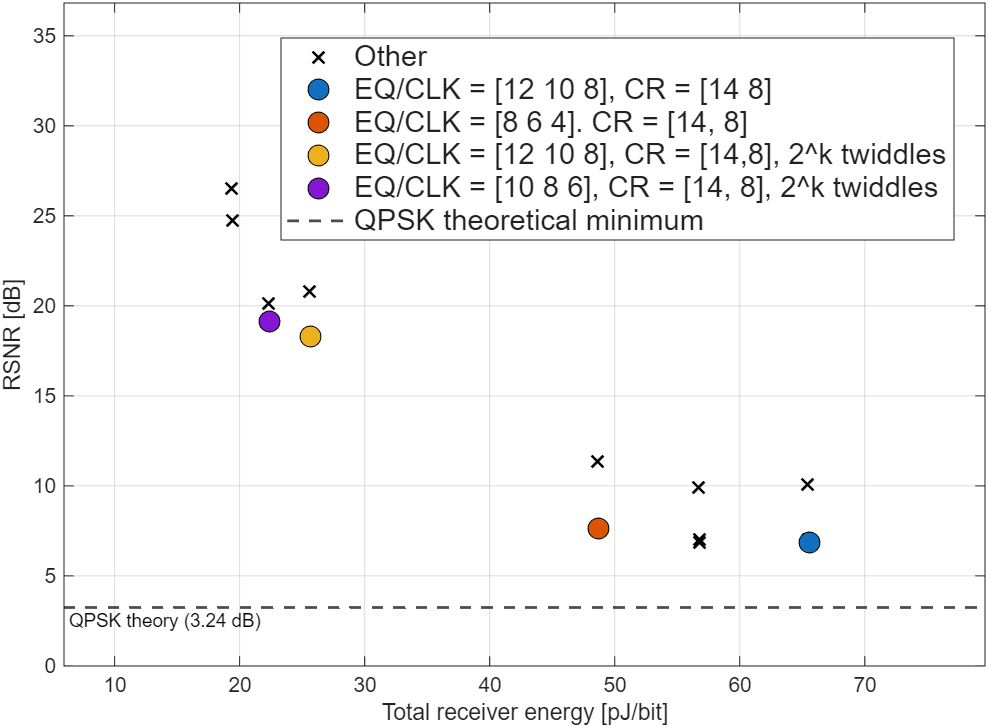
\includegraphics[width=0.65\textwidth]{RSNR vs receiver energy.png}
    \caption{RSNR (dB) vs receiver energy (pJ/bit) for each implementation at ENOB = 6. EQ/CLK is the equalisation/clock recovery block with precisions shown for [static equaliser, timing error estimate, adaptive equaliser]. CR is the carrier recovery block with precisions shown for [frequency recovery, phase recovery].}
    \label{fig:RSNR_energy}
\end{figure}

\subsection{Receiver Energy Breakdown}
\Cref{fig:rx_energy_breakdown} shows the energy contributed by each group of DSP blocks for the highlighted operating points. Carrier recovery comprises CFO estimation, phase-error estimation, and phase correction; equalisation comprises the static and adaptive equalisers; and the front end comprises the ADC, orthogonalisation, and deskew, all operating at 6 bits. Equalisation dominates the receiver energy, almost entirely through the static equaliser, so reducing its precision or simplifying it with $2^k$ twiddle-factor rounding has the largest impact on receiver energy. Clock recovery is the next largest contributor, which is why a low-complexity detector such as the Modified Godard TED is essential in an energy-efficient design. The front end and carrier recovery contribute least: carrier recovery benefits from amortising its estimates over many symbols and from efficient CORDIC phase corrections, while orthogonalisation is similarly amortised and the known, static I/Q skew allows a short deskew interpolator.
\begin{figure}[H]
    \centering
    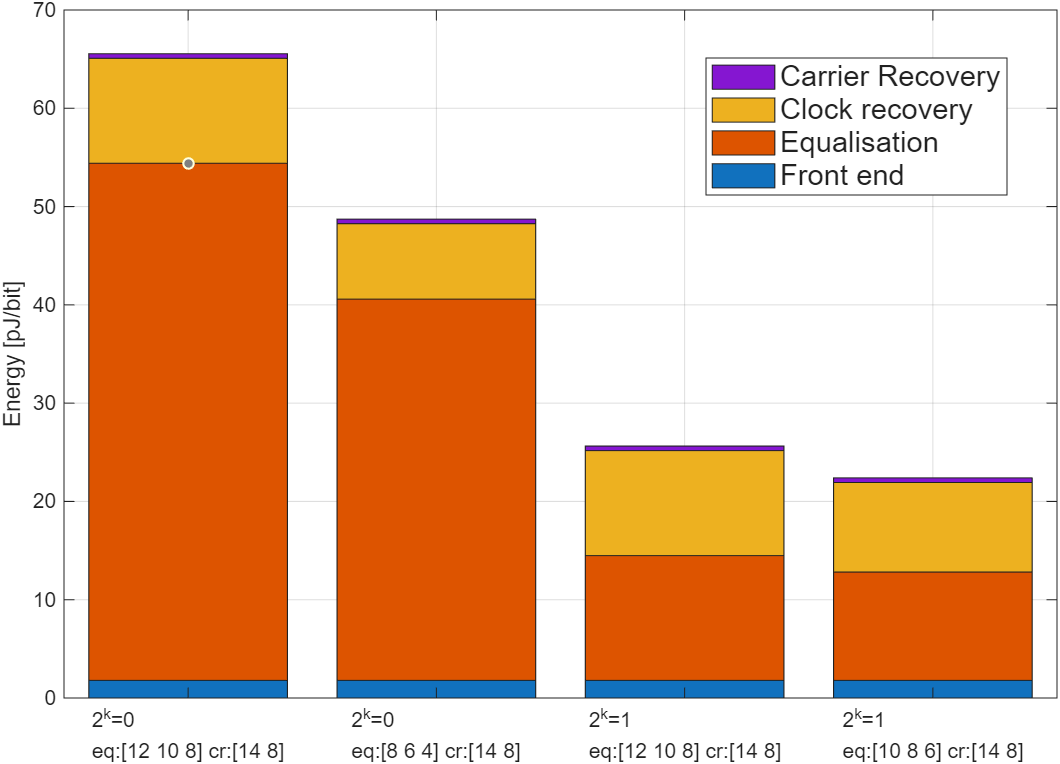
\includegraphics[width=0.7\textwidth]{final_rx_energy.png}
    \caption{Energy breakdown of the receiver for highlighted operating points in \cref{fig:RSNR_energy}.}
    \label{fig:rx_energy_breakdown}
\end{figure}

\subsection{Transmitter vs Receiver Energy}
The RSNR differences translate into transmitter energy through the energy model of \cref{chapter:energy}, in which the transmitter efficiency was found to be $\approx 10\,\%$. \Cref{tab:tx_rx_energy} reports the transmitter, receiver, and combined system energy per bit, with the corresponding power consumption, for the highlighted operating points of \cref{fig:RSNR_energy}. The transmitter energy is far smaller than the receiver energy at every operating point: the receiver consumes power of order 1\,W while the transmitter draws only a few milliwatts. These figures are useful for comparison but do not capture every source of consumption: the analogue front-end and laser-driver electronics, thermal control, and clock distribution are not modelled, and the 14\,nm arithmetic-energy model is extrapolated from older process data, so the true receiver energy is likely lower. Within this model the receiver energy dominates the combined total, so the large receiver saving from $2^k$ twiddle-factor rounding far outweighs its small increase in transmitter energy, making it worthwhile in an energy-efficient coherent receiver.

\begin{table}[H]
    \centering
    \caption{Transmitter, receiver, and combined system energy per bit and the corresponding power consumption for the highlighted operating points of \cref{fig:RSNR_energy}. All points use a carrier-recovery precision of $[14,8]$; the equaliser precision is given as $[\text{Static},\text{Clk},\text{Adaptive}]$ fractional bits and $2^k$ denotes power-of-two FFT twiddles.}
    \label{tab:tx_rx_energy}
    \begin{tabular}{ccccccccc}
        \toprule
        \multirow{2}{*}{$2^k$} & \multirow{2}{*}{EQ/CLK Precision [bits]} & \multicolumn{3}{c}{Energy (pJ/bit)} & \multicolumn{3}{c}{Power (W)} \\
        \cmidrule(lr){3-5}\cmidrule(lr){6-8}
         & & $E_\mathrm{tx}$ & $E_\mathrm{rx}$ & $E_\mathrm{sys}$ & $P_\mathrm{tx}$ & $P_\mathrm{rx}$ & $P_\mathrm{sys}$ \\
        \midrule
        off & $[12,10,8]$ & $0.020$ & $65.55$ & $65.57$ & $0.0012$ & $3.999$ & $4.000$ \\
        off & $[8,6,4]$   & $0.023$ & $48.73$ & $48.75$ & $0.0014$ & $2.972$ & $2.974$ \\
        on  & $[12,10,8]$ & $0.279$ & $25.64$ & $25.91$ & $0.0170$ & $1.564$ & $1.581$ \\
        on  & $[10,8,6]$  & $0.340$ & $22.40$ & $22.74$ & $0.0208$ & $1.366$ & $1.387$ \\
        \bottomrule
    \end{tabular}
\end{table}

% =====================================================================
\chapter{Conclusion}\label{chapter:conclusion}
% =====================================================================
This report investigated the design of an energy-efficient digital signal processing receiver for a coherent passive optical network, with the aim of identifying which algorithms and arithmetic precisions reduce energy consumption while still meeting the CPON performance requirements. Each stage of the receiver was implemented in both floating and fixed point and the stages were combined into a complete pipeline, so that the algorithm and precision choices could be assessed together rather than in isolation.

\section{Summary of Findings}
A bit-accurate fixed-point model of the receiver was developed and compiled to an executable form. This allowed the energy of each block to be estimated from its real operation counts and word lengths rather than from algorithmic complexity alone, and, more usefully, allowed the effect of quantisation error on the bit-error rate to be measured directly rather than assumed. The required SNR (RSNR) to reach the FEC threshold was adopted as the common figure of merit, so that the cost of a coarser, lower-energy implementation could be expressed as an SNR penalty and weighed against its energy saving.

Throughout the receiver, the algorithms commonly used in long-haul coherent systems were compared against simpler alternatives better suited to a short-reach, energy-constrained access network. For chromatic-dispersion equalisation and timing recovery, an overlap-save frequency-domain equaliser was paired with a Modified Godard timing-error detector that reuses the same FFT, avoiding the cost of a separate timing loop, and the FFT twiddle factors could optionally be rounded to powers of two to remove their multiplications. For frequency recovery, the data-aided differential-phase-and-Kay estimator required far fewer operations than a Rife \& Boorstyn FFT search while reaching an acceptable residual offset when averaged over a modest number of subframes. For phase recovery, a pilots-only correction performed almost identically to the Viterbi \& Viterbi algorithm across the linewidth range of interest, at a fraction of the cost. In each case the simpler algorithm was retained, as the small performance gap did not appear to justify the additional energy.

Sweeping the fixed-point precision of each stage identified the lowest word lengths at which the blocks still operate, and these minimum-precision operating points were combined and tested in the full pipeline. The energy breakdown showed that equalisation, and the static equaliser in particular, dominates the receiver energy, so power-of-two twiddle rounding and reductions in equaliser precision have the largest effect on the total. Converting the RSNR of each implementation into a transmitter energy through a shot-noise network model indicated that, at the operating points considered, the transmitter energy is small compared with the receiver energy, so the combined system energy is dominated by the receiver. Under this model the energy saved by the power-of-two twiddle factors outweighed the modest increase in transmitter energy caused by their SNR penalty, though this result is specific to the assumed efficiencies and network parameters.

\section{Challenges}
Working in fixed point introduced failure modes that do not arise in floating-point development and that often produce plausible but incorrect results rather than obvious errors. Particular care was therefore taken when converting quantities between fixed-point formats, where a mismatched word length or binary point silently rescales or truncates a signal, and at points where intermediate values could overflow their range. Each block's fixed-point output was checked against its floating-point reference to catch these effects, and the word lengths and binary points were set explicitly at every stage rather than relying on default casting.

The fixed-point simulations were also far slower than their floating-point equivalents, as evaluating fixed-point objects through the MATLAB interpreter carries a large per-operation overhead. With the precision sweeps requiring many Monte Carlo trials across a range of SNRs, this run time became the main constraint on how much could be explored. It was overcome by compiling each fixed-point block directly to a native executable with MATLAB Coder rather than running it through the interpreter, which reduced the run time of the sweeps by a large factor and made the full-pipeline experiments feasible.

\section{Limitations and Further Work}
The energy figures in this report are best read as a means of comparing implementations rather than as absolute estimates. The model counts only the energy of the arithmetic operations in each block, using coefficients extrapolated from a 45\,nm process to a 14\,nm node, and it omits several sources of dissipation present in a real receiver, including clocking, on-chip memory and data movement, the analogue front end, and the laser-driver and thermal-management electronics. It is also not cycle-accurate: there is no model of the clock, pipelining, or parallelism that a hardware implementation requires, so quantities such as throughput and latency could not be assessed. The network model is similarly simplified, assuming a flat loss and a shot-noise-limited link, and the front-end imperfections corrected by orthogonalisation and deskew were taken to be ideal in the bit-error simulation.

An FPGA model was not developed within the timeframe of this project, and two extensions would address the largest of the limitations above. The first would be to implement the fixed-point blocks on an FPGA or in a hardware simulator targeting a modern process node, giving a cycle-accurate energy estimate from place and route that includes clocking and memory and reflects current technology. The second would be to build a more detailed network model in which transmit power, link loss, and the resulting received SNR are related explicitly, allowing the transmitter and receiver energy trade-off to be examined across realistic operating conditions rather than at the single worst-case point considered here.

\renewcommand*{\bibfont}{\footnotesize}
\setlength{\bibitemsep}{0pt}
\defbibheading{compact}[\bibname]{%
    \clearpage
    \addcontentsline{toc}{chapter}{#1}%
    \markboth{#1}{#1}%
    \noindent{\Huge\bfseries #1}\par\vspace{0.8em}%
    \enlargethispage{3\baselineskip}%
}
\printbibliography[heading=compact]

% =====================================================================
\appendix


% =====================================================================
\chapter{Modified Cramer-Rao Bound for Frequency Estimation}\label{appendix:mcrb}
% =====================================================================
\section{The Cramer-Rao and Modified Cramer-Rao Bounds}
The Cramer-Rao bound (CRB) sets a lower limit on the variance of any unbiased estimator of a parameter from noisy observations. For a scalar parameter $\lambda$ estimated from an observation $\mathbf{r}$ with likelihood $p(\mathbf{r}\mid\lambda)$,
\begin{equation}
    \operatorname{var}(\hat\lambda) \ge \mathrm{CRB}(\lambda) = \frac{1}{J(\lambda)}, \qquad J(\lambda) = \mathbb{E}_{\mathbf r}\!\left[\left(\frac{\partial \ln p(\mathbf r\mid\lambda)}{\partial\lambda}\right)^2\right],
\end{equation}
where $J(\lambda)$ is the Fisher information: a measure of how sharply the likelihood depends on $\lambda$, and hence how precisely $\lambda$ can be inferred from the data.

In the carrier-recovery problem the received samples depend not only on the CFO but also on the unknown transmitted symbols (and, in blind operation, the phase noise). These are nuisance parameters $\mathbf u$: unwanted, but still shaping the likelihood. The exact CRB then requires the marginal likelihood $p(\mathbf r\mid\lambda) = \int p(\mathbf r\mid\lambda,\mathbf u)\,p(\mathbf u)\,\mathrm d\mathbf u$, the average over all possible nuisance values, which is generally intractable.

The modified Cramer-Rao bound (MCRB) sidesteps this by instead averaging the \emph{conditional} Fisher information, computed with the nuisance parameters known, over their distribution \cite{Andrea1994}:
\begin{equation}
    \mathrm{MCRB}(\lambda) = \frac{1}{\mathbb E_{\mathbf u}\!\left[ J(\lambda\mid \mathbf u)\right]}, \qquad J(\lambda\mid\mathbf u) = \mathbb E_{\mathbf r\mid \mathbf u}\!\left[\left(\frac{\partial \ln p(\mathbf r\mid\lambda,\mathbf u)}{\partial\lambda}\right)^2\right].
\end{equation}
Knowing the nuisance parameters can only add information, so the MCRB is a looser bound than the CRB, $\mathrm{MCRB}\le\mathrm{CRB}\le\operatorname{var}(\hat\lambda)$. It is far easier to evaluate, however, and coincides with the CRB at high SNR, which makes it the natural benchmark for the frequency estimators.

\section{Use in CFO Estimation}
For frequency recovery the parameter of interest is the normalised CFO $\nu = f_d/R_s$ and the nuisance parameters are the data symbols. The MCRB gives the smallest variance with which $\nu$ can be estimated from $L$ symbols at a given SNR, independent of the particular algorithm. An estimator is (asymptotically) efficient if its variance reaches the MCRB; the SNR at which it begins to depart from the bound is the threshold SNR used throughout \cref{chapter:carrier_recovery} to compare the Rife \& Boorstyn and differential phase and Kay estimators (\cref{fig:fft_mcrb_data,fig:diffkay_data}). Plotting the measured normalised MSE against the MCRB therefore shows both how close each estimator comes to the fundamental limit and the SNR range over which it remains usable.


\chapter{Risk Assessment}\label{chapter:risk_assessment}
The hazards identified at the beginning of this project were computer use and potential use of class 1M lasers. I was not exposed to any class 1M lasers during the project as the work was done on a computer simulation. Hazards associated with computer use were mitigated with correct posture and regular breaks.

\end{document}
